\documentclass[a4paper]{article}

% CJK support: prefer ctex, fallback to XeTeX native line breaking
\IfFileExists{ctex.sty}{
  \usepackage[fontset=fandol]{ctex}
}{
  \usepackage{fontspec}
  \XeTeXlinebreaklocale "zh"
  \XeTeXlinebreakskip = 0pt plus 1pt
  \IfFontExistsTF{Songti SC}{\setmainfont{Songti SC}}{%
    \IfFontExistsTF{Noto Serif CJK SC}{\setmainfont{Noto Serif CJK SC}}{}%
  }
  \IfFontExistsTF{Heiti SC}{\setsansfont{Heiti SC}}{%
    \IfFontExistsTF{Noto Sans CJK SC}{\setsansfont{Noto Sans CJK SC}}{}%
  }
}

% Basic packages
\usepackage{amsmath, amssymb}
\usepackage{graphicx}
\usepackage[margin=2.5cm]{geometry}
\emergencystretch=3em
\usepackage[most]{tcolorbox}
\usepackage{etoolbox}
\usepackage{listings}
\usepackage{hyperref}
\hypersetup{hidelinks,pdftitle={南京大学生成式软件工程第11讲：软件质量保障 (1)},pdfauthor={lecture-to-notes}}
\usepackage{booktabs}
\usepackage{subcaption}
\usepackage{float}
\usepackage{tikz}
\IfFileExists{pgfplots.sty}{
    \usepackage{pgfplots}
    \pgfplotsset{compat=1.18}
}{}

% ===== Highlight boxes =====
\newtcolorbox{knowledgebox}[1]{
    enhanced, colback=black!2!white, colframe=black!65, colbacktitle=black!65,
    coltitle=white, fonttitle=\bfseries, title={#1}, attach boxed title to top left={yshift=-2mm, xshift=2mm},
    boxrule=1pt, sharp corners
}

\newtcolorbox{importantbox}[1]{
    enhanced, colback=red!3!white, colframe=red!45!black, colbacktitle=red!45!black,
    coltitle=white, fonttitle=\bfseries, title={#1}, sharp corners
}

\newtcolorbox{warningbox}[1]{
    enhanced, colback=red!5!white, colframe=red!75!black, colbacktitle=red!75!black,
    coltitle=white, fonttitle=\bfseries, title={#1}, sharp corners
}

% ===== Code listings =====
\lstset{
    basicstyle=\ttfamily\small,
    keywordstyle=\color{blue},
    stringstyle=\color{red!60!black},
    commentstyle=\color{green!60!black},
    breaklines=true,
    frame=single,
    numbers=left,
    numberstyle=\tiny\color{gray},
    captionpos=b,
    extendedchars=false
}

% ===== Figure provenance and unit macros =====
\newcommand{\vtag}{\protect\footnotemark}
\newcommand{\srcnote}[1]{\footnotetext{视频画面时间区间：#1。若为裁剪图，时间区间仍对应原视频画面。}}
\newcommand{\degC}{\ensuremath{^{\circ}\mathrm{C}}}
\newcommand{\um}{\ensuremath{\mu\mathrm{m}}}
\newcommand{\nm}{\ensuremath{\mathrm{nm}}}
\newcommand{\angstrom}{\ensuremath{\text{\AA}}}

% ===== Front-page metadata =====
\newcommand{\notetitle}{软件质量保障 (1)}
\newcommand{\notesubtitle}{南京大学生成式软件工程 · 第 11 讲}
\newcommand{\noteauthors}{中文课程讲义 · lecture-to-notes}
\newcommand{\notedate}{2026 年 11 月 3 日}
\newcommand{\videochannel}{蒋炎岩主讲 / 绿导师原谅你了上传}
\newcommand{\videopublishdate}{20261103}
\newcommand{\videoduration}{97 分 07 秒}
\newcommand{\videourl}{https://www.bilibili.com/video/BV1ej4g6xESc/}
\newcommand{\videocoverpath}{cover.jpg}

\begin{document}

% ===== Title page =====
\begin{titlepage}
\centering
{\Large 课程笔记\par}
\vspace{1.2cm}
{\huge\bfseries \notetitle\par}
\ifdefempty{\notesubtitle}{}{
\vspace{0.3cm}
{\large \notesubtitle\par}
}
\vspace{0.5cm}
{\large \noteauthors\par}
\vspace{0.3cm}
{\large \notedate\par}
\vspace{1.0cm}

\ifdefempty{\videocoverpath}{
{\small 请在生成笔记时填入视频封面图的本地路径。\par}
}{
\includegraphics[width=0.82\textwidth,height=0.40\textheight,keepaspectratio]{\videocoverpath}\par
}

\vfill
\begin{tcolorbox}[width=0.9\textwidth, colback=black!2!white, colframe=black!60, sharp corners]
\textbf{视频作者/频道}：\videochannel\par
\textbf{发布日期}：\videopublishdate\par
\textbf{视频时长}：\videoduration\par
\textbf{视频链接}：\ifdefempty{\videourl}{待填写}{\url{\videourl}}\par
\end{tcolorbox}
\end{titlepage}

% ===== Executive Summary =====
\newpage
\section*{执行摘要与核心脉络}

本讲义对应南京大学 2026 年秋季学期《生成式软件工程》（Generative Software Engineering）第 11 讲《软件质量保障 (1)》，由蒋炎岩老师主讲。在上一讲剖析了大型软件系统（如航空母舰与 \texttt{DeepSeek Harness}）如何沿时间维度增量演化之后，本讲直面“许愿编程”（Vibe Coding）时代最尖锐的工程矛盾：\textbf{当向大模型许愿即可在几分钟内生成上千行看似“能跑”的代码时，为什么人类反而更容易失去对软件的掌控？面对意图、规约与实现之间的两道鸿沟（\texttt{intent-spec-impl gap}），我们应当如何建立一套从第一性原理出发的软件质量保障体系？}

全讲围绕九个环环相扣的核心模块展开：
\begin{enumerate}
    \item \textbf{从“能运行”到“能驾驭”——演化视角下的自动化的反讽}：回顾第 10 讲航母演化隐喻与五六十万行至 100万行级工业代码库的认知门槛，剖析 \texttt{intent-spec-impl gap}。指出“许愿编程”带来的最大隐患是人类只看到软件的表象而丧失对其内部逻辑的掌控；借用 Bainbridge（1983）提出的\textbf{“自动化的反讽”（Ironies of Automation）}，阐明当日常编码交给机器后，人类练手机会减少，但在系统异常崩溃时接管兜底所需的工程本领反而更高。
    \item \textbf{任何程序员都有“幻觉”——从手滑 Typo 到双层循环的未定义行为}：对比大模型编码基准与人类“古法编程”现实，指出人类程序员的幻觉往往比 AI 更大。从 10年（11年）前风靡 GitHub 的命令行纠错工具 \texttt{thefuck}，到双层 \texttt{for} 循环将内层 \texttt{j++} 误写为 \texttt{i++} 的经典手滑案例，结合课堂板书完整推演该缺陷为何在 $n > 0$ 时导致内层循环死锁、有符号整数 \texttt{i} 递增溢出并触发 C 语言未定义行为（Undefined Behavior，UB）。
    \item \textbf{软件质量的三元模型——Fault、Error 与 Failure}：系统建立软件质量保障的理论基石——静态代码缺陷（\textbf{Fault}）、运行时偏离规约的内部错误状态（\textbf{Error}）与观察边界上可感知的外部失效（\textbf{Failure}）。剖析为何 \texttt{Fault $\to$ Error} 与 \texttt{Error $\to$ Failure} 两个箭头均非必然，并通过 1996 年阿丽亚娜 5 号（Ariane 501）火箭首飞解体事故（64 位浮点数转 16位有符号整数缺少越界保护，且主备惯导复制同一套软硬件导致共模失效），揭示冗余备份设计与观察边界选择的铁律。
    \item \textbf{质量保障的双轮驱动——测试（Testing）与断言（Assertion）}：在状态空间几何图景下阐明两大基本手段的正交分工：\textbf{测试}负责在规约输入空间中采样，推动 \texttt{Fault $\to$ Error}；\textbf{断言}负责在运行时即时检查不变量（Invariant），推动 \texttt{Error $\to$ Failure}。对比 Java（消除指针 UB）与 Safe Rust（消除内存安全问题）的语言级防线，剖析 C 语言指针解引用、\texttt{malloc/free} 生命周期与 Linux 内核 \texttt{goto} 集中清理范式。
    \item \textbf{“在我机器上能跑”说明了什么——广义输入空间与 SWE-agent 反馈闭环}：拆解“运行 100次、1000次、1万次”背后的环境差异（\texttt{package.json} 与 \texttt{package-lock.json} 依赖锁文件的能力边界）与非确定性输入维度（系统负载、\texttt{gettimeofday()} 在 $T+1\text{秒}$ 或 $T+1\text{毫秒}$ 的分叉、网络延迟、CHESS 主动探索的并发线程调度交错）。结合 Dijkstra（1972）名言与伪排序函数在 $n$ 元随机排列上碰巧蒙对的 $1/n!$ 极小概率，解释为何测试依然极具威力，并精读 2024年 \texttt{SWE-agent} 论文的人机接口（ACI）闭环。
    \item \textbf{经典软件工程测试体系——四个层次、黑盒/白盒设计与日常工程化}：梳理 100万行级系统的四个测试层次（单元、集成、系统、验收）及 1999 年 NASA 火星气候轨道器（Mars Climate Orbiter）因英制 $\mathrm{lbf\cdot s}$ 与公制 $\mathrm{N\cdot s}$ 单位失配（相差约 $4.45$ 倍）坠毁的教训；详解黑盒测试（等价类、边界值、决策表、状态转换）与白盒测试（语句/分支/路径覆盖率达到 100\% 仍可能因缺乏正确 Test Oracle 而漏掉 \texttt{add(a,b) = a - b}），辅以“测试工程师进酒吧”漫画、测试金字塔、Stub/Mock 替身、回归测试（先失败后通过）与持续集成（CI）。
    \item \textbf{真实系统的长程任务挑战——从许愿 CS:GO（CS:THREE）到可测试性架构}：现场演示向智能体许愿开发的浏览器 3D 战术射击游戏 \texttt{CS:THREE}（累计 202 次提交、12 个里程碑、4,021 行代码、跑 12秒看 AI 交火），复盘智能体因疯狂多机位截图塞满上下文直至触发 HTTP \texttt{413 Payload Too Large} 的轨迹教训。由此提炼出全讲核心命题——\textbf{架构决定了软件质量}：通过模块化边界、无状态纯函数（Pure Functions）、时钟与随机数显式注入、Stripe 幂等键（Idempotency Key）以及 FoundationDB（模拟 100台服务器集群故障）的确定性仿真，让复杂系统变得可控制、可重放、可局部验证。
    \item \textbf{灵光一闪（一）：差分测试（Differential Testing）——从 NEMU 到香山处理器}：回顾 2013年主讲教师在南京大学创立 NEMU 教学模拟器时如何受《仙剑奇侠传》跑飞启发，提出让待测实现与参考实现（QEMU/Spike/NEMU）逐指令比对状态的 \textbf{DiffTest} 方法，并展示该方法在开源 RISC-V 处理器“香山”（XiangShan）中运行 4 亿（$4 \times 10^8$）个时钟周期后精准捕获 \texttt{mstatus} 控制状态寄存器（CSR）不一致的工业级威力。
    \item \textbf{灵光一闪（二）：模糊测试（Fuzz Testing）与跳出屏幕的硬件闭环}：回顾过去 30年软件工程在自动测试生成上的求索，剖析 AFL（American Fuzzy Lop）如何将输入空间搜索转化为带边覆盖（Edge Coverage）选择压力的遗传演化算法；最后以 Android 初创团队工程师 San Mehat 打造 3D 打印舵机自动插拔 SD 卡机器人、以及主讲教师用 5厘米 $\times$ 5厘米四帧光栅画钥匙扣许愿的生动案例收束全讲。
\end{enumerate}

\newpage
\tableofcontents
\newpage

% =========================================================================
% SECTION 1
% =========================================================================
\section{从“能运行”到“能驾驭”：软件演化视角下的质量困局}

\subsection{回顾：航母是怎么造出来的与两道工程鸿沟}

在上一讲（第 10 讲《软件的演化：航母是怎么造出来的》）中，我们探讨了一个令所有计算机科学学生感同身受的现象：当你直接走上一艘现代航空母舰，或者从 GitHub 上把 Linux 内核、现代编译器、工业级数据库、大型应用服务器的代码仓库 \texttt{git clone} 下来时，面对五六十万行乃至 100万行以上的代码，你的第一反应往往是彻底的眩晕与无从下手。哪怕项目的 \texttt{README.md} 写得再清晰，一旦深入源码目录，盘根错节的模块依赖、各种匪夷所思的边界特判与历史兼容分支就会扑面而来。

\begin{figure}[H]
\centering
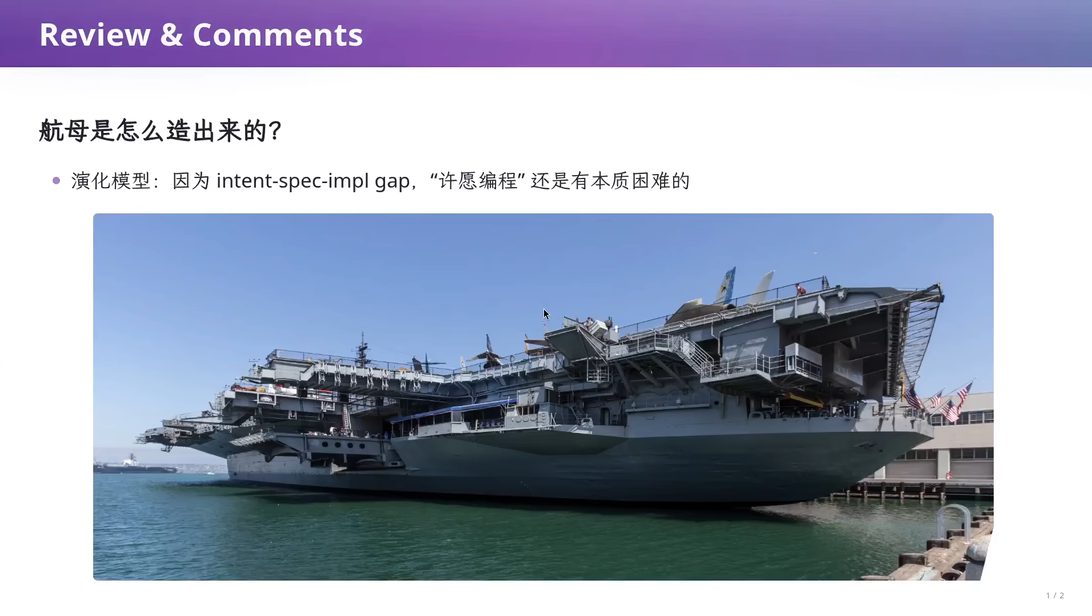
\includegraphics[width=0.92\textwidth]{figures/fig_01_review_carrier_evolution.png}
\caption{课程回顾：航母是如何造出来的？演化模型揭示了由于 \texttt{intent-spec-impl gap} 的存在，“许愿编程”依然面临本质困难\vtag}
\end{figure}
\srcnote{00:00:45--00:01:00}

为什么工业级系统一定会演化得像航母一样复杂？因为真实世界的需求从来不是静态的。正如航母不仅要能航行，还要能起降固定翼战机、要在恶劣海况与战损下容错、要协同调度数千名舰员一样，工业级软件在长期演化过程中不断叠加新的业务需求、性能约束与安全防御。在这个过程中，软件工程始终横亘着两道本质鸿沟（\textbf{\texttt{intent-spec-impl gap}}）：

\begin{equation}
\text{Intent（真实意图）}
\;\xrightarrow{\;\text{Intent--Spec Gap}\;}\;
\text{Spec（系统规约）}
\;\xrightarrow{\;\text{Spec--Impl Gap}\;}\;
\text{Impl（代码实现）}
\end{equation}

上式中各组成部分的工程含义如下：
\begin{itemize}
    \item $\text{Human Intent}$（人类真实意图）：用户或架构师脑海中希望软件达成的目标（例如“做一个好玩的战术射击游戏”或“构建一个可靠的选课系统”），它往往是模糊、不完整甚至自相矛盾的；
    \item $\text{Specification}$（系统规约，简称 Spec）：对软件在各种输入与环境条件下“应当做什么、不应当做什么”的精确契约定义；从意图到规约的鸿沟（$\text{Gap 1}$）是需求工程与架构演化的核心挑战；
    \item $\text{Implementation}$（代码实现，简称 Impl）：由人类程序员或编码智能体（Coding Agent）实际编写出的可执行代码；从规约到实现的鸿沟（$\text{Gap 2}$）——即\textbf{“我们怎样知道写出来的代码真正符合规约？当代码违背规约时，我们怎样尽早发现并定位它？”}——正是本讲《软件质量保障》的核心主题。
\end{itemize}

\subsection{从能理解的历史时刻 Rebase 与“自动化的反讽”}

面对五六十万行代码的庞然大物，上一讲给出了一个极具威力的工程心智工具——\textbf{从历史开始“Rebase”}（图 2）。一艘现代核动力航母看似不可思议，但如果我们把时间轴拨回 1922 年美国海军的第一艘航母“兰利号”（USS Langley，CV-1），就会发现它不过是在一艘运煤船（USS Jupiter）的船体上拆掉运煤桁架、铺上一层木质飞行甲板改装而成的。当你理解了“运煤船 $+$ 一层平板 $=$ 初代航母”这个最简初态（Initial Commit），再沿着历史提交记录（Git Log）一步步观察升降机、机库、弹射器、斜角甲板是如何随着飞机重量与速度的增长而被逼出来的，整座航母的复杂度就瞬间变得清澈可解。

\begin{figure}[H]
\centering
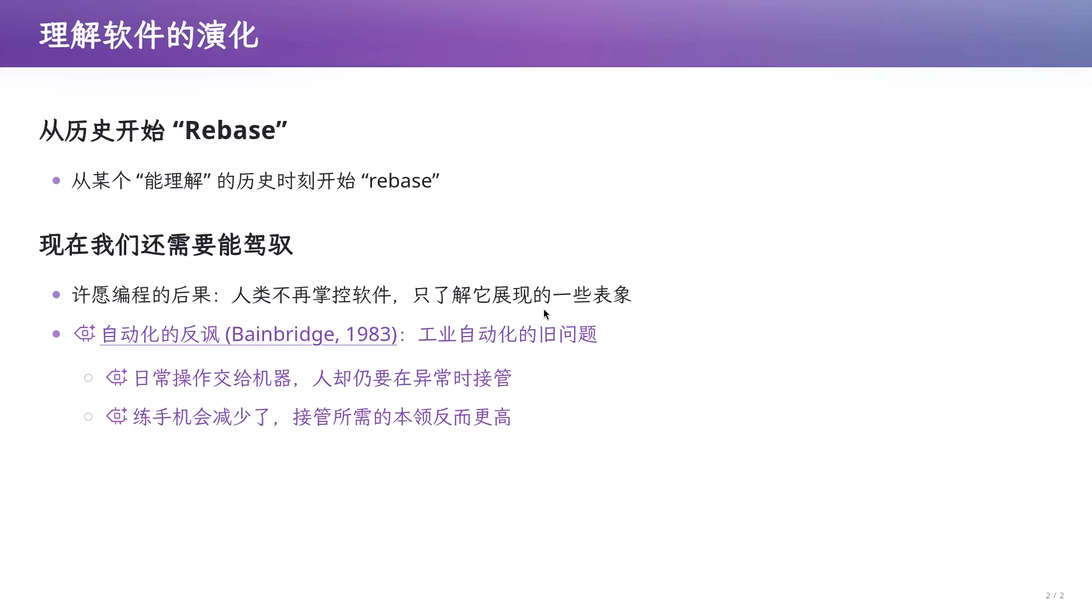
\includegraphics[width=0.92\textwidth]{figures/fig_02_rebase_ironies_of_automation.png}
\caption{理解软件的演化：从某个“能理解”的历史时刻开始 Rebase，并警惕 Bainbridge（1983）提出的“自动化的反讽”\vtag}
\end{figure}
\srcnote{00:03:45--00:04:00}

然而，在今天的大模型与“许愿编程”（Vibe Coding）时代，这种建立在演化历史之上的掌控力正在面临前所未有的危机。主讲教师在课堂终端中展示了真实软件仓库的提交历史（图 3），并指出一个令人警醒的事实：

\begin{figure}[H]
\centering
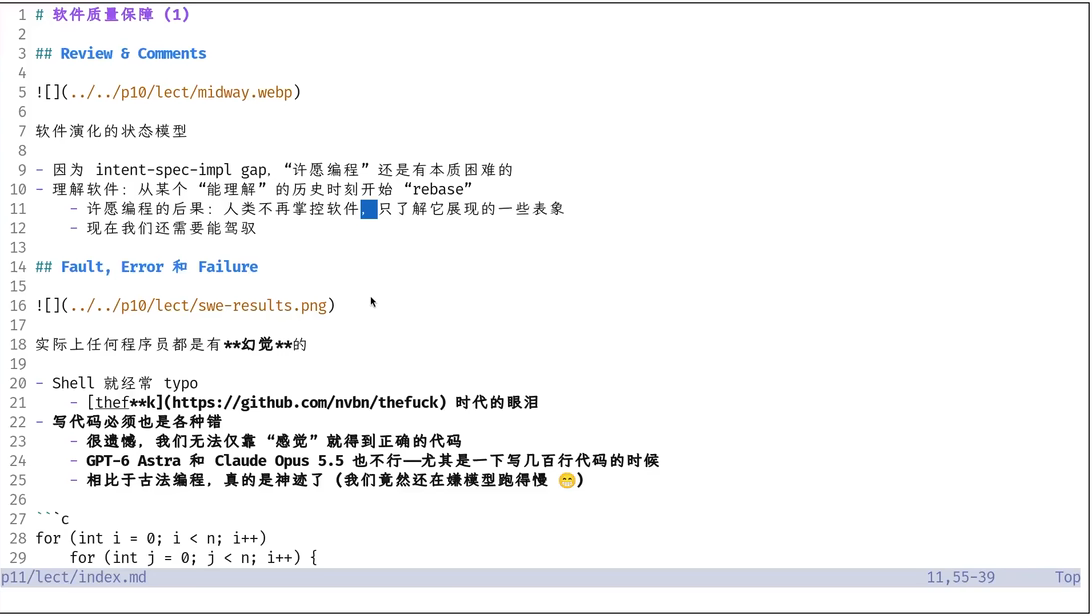
\includegraphics[width=0.92\textwidth]{figures/fig_03_git_history_terminal.png}
\caption{命令行演示：软件仓库的提交历史与演化轨迹，是人类理解并驾驭复杂系统的关键线索\vtag}
\end{figure}
\srcnote{00:07:00--00:07:15}

当你向 Coding Agent 许下愿望（例如“帮我写一个带权限控制与并发选课功能的教务后端”），Agent 哗啦啦一下子吐出几千行甚至上万行代码。你满怀欣喜地执行启动命令，浏览器里弹出了精美的界面，点几下按钮也能正常跳转——\textbf{它“能运行”（It works on the surface），但你完全不再“掌控”它（You are no longer in control）}！你只看到了软件展现出来的几个表象，却根本不知道它在数据库事务锁、异常回滚、边界溢出和并发竞争上埋下了多少定时炸弹。

这并非人工智能时代独有的新问题，而是工业自动化历史上反复上演的经典困境。早在 1983 年，认知心理学家 Lisanne Bainbridge 就在其发表于 \textit{Automatica} 的经典论文《Ironies of Automation》（自动化的反讽）中深刻指出了这一悖论：

\begin{importantbox}{核心概念：自动化的反讽（Ironies of Automation, Bainbridge 1983）}
工业界引入自动化系统的初衷，是因为觉得人类操作员容易疲劳、容易犯错，希望用机器替代人的日常操作。但只要自动化系统还不是 100\% 绝对完美，它就会陷入两个辛辣的“反讽”：
\begin{enumerate}
    \item \textbf{日常操作交给机器，人类却仍要在最棘手的异常时刻接管兜底}：机器接管了所有简单、常规、顺畅的工况；一旦机器遇到超出其设计边界的极端异常而报警停机时，系统会瞬间把控制权甩回给人类操作员。
    \item \textbf{练手机会变少了，接管所需的本领反而更高了}：人类工程师原本正是通过每天处理大量日常中低难度的编码与调试任务，才建立起对系统内部状态机的肌肉记忆与直觉；当日常编码全部交给 Agent 代劳后，人类丧失了日常构建心智模型的机会，却被要求在几万行陌生代码发生诡异崩溃时一剑封喉地完成救火——这在工程上是根本不可能持续的。
\end{enumerate}
\end{importantbox}

因此，即使在 Agent 可以替我们编写 99\% 代码的今天，只要最终对系统可用性、安全性与商业后果承担责任的依然是人类工程师，我们就绝不能停留在“能跑就行”的许愿阶段，而必须掌握一套能够\textbf{检验、约束并驾驭软件质量}的硬核工程方法。

\begin{knowledgebox}{工程心智工具：如何对陌生或 AI 生成的系统做“认知 Rebase”？}
面对五六十万行历史代码或 Agent 一次性生成的数千行代码，切忌直接扎进细节大海：
\begin{enumerate}
    \item \textbf{寻找最简可理解初态（Base Commit）}：剥离所有缓存、并发优化与复杂容错，先找出系统最初那条核心主干（如同“运煤船加一层木甲板”）；
    \item \textbf{沿增量提交逐层叠加约束}：把每一次架构复杂度跃迁都还原为“为了解决哪一个具体的失效（Failure）或规约边界而引入的最小增量 $\Delta$”，从而夺回对系统的掌控权。
\end{enumerate}
\end{knowledgebox}

\subsection{本章小结}

本章从航母演化隐喻出发，区分了 \texttt{Intent-Spec} 与 \texttt{Spec-Impl} 两道鸿沟，结合 Bainbridge（1983）“自动化的反讽”指出：许愿编程越是让生成代码变得廉价，人类工程师就越需要依靠系统的质量保障体系来维持对复杂软件的真正掌控。

% =========================================================================
% SECTION 2
% =========================================================================
\section{任何程序员都有“幻觉”：从手滑 Typo 到未定义行为}

\subsection{大模型的编码神迹与人类“古法编程”的幻觉}

在日常讨论大模型（LLM）时，人们最常挂在嘴边的批评就是“AI 有幻觉（Hallucination）”——比如编造不存在的 API、写错循环边界或漏掉空指针检查。但蒋老师在课堂上展示了一张大模型编码基准评测图表（图 4），并提出了一个振聋发聩的反问：\textbf{相比于人类延续了几十年的“古法编程”（手敲代码），今天的大模型在短短几十秒内生成数百行语法正确、逻辑大体自洽的代码，简直已经是神迹了；而人类程序员写代码时的“幻觉”，其实远远比 AI 严重得多！}

\begin{figure}[H]
\centering
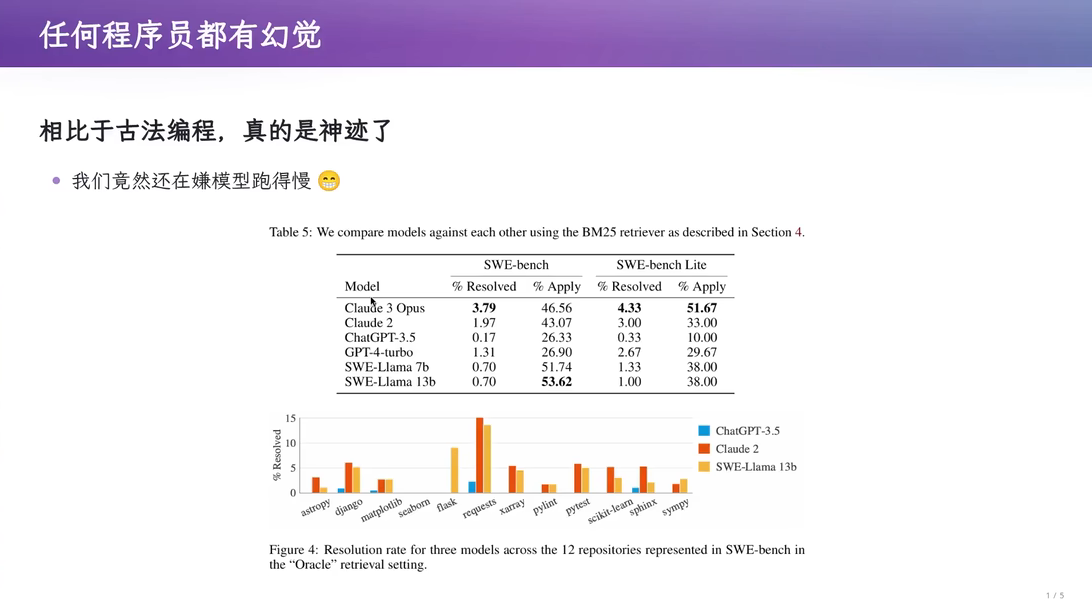
\includegraphics[width=0.92\textwidth]{figures/fig_04_programmer_hallucination_bench.png}
\caption{任何程序员都有幻觉：相比于人类古法编程，现代大模型在编码基准上的表现已堪称神迹，但我们竟然还在嫌模型跑得慢\vtag}
\end{figure}
\srcnote{00:08:30--00:08:45}

为什么说人类程序员充满幻觉？因为人类不仅在理解复杂规约时会产生认知偏差，甚至在把脑子里的清晰想法敲进键盘的瞬间，手指都会不听使唤地“手滑”（Typo）。

主讲教师在课堂上打开了一个 10年（准确地说是 11年）前在 GitHub 上斩获数万 Star 的传奇开源项目——\texttt{nvbn/thefuck}（图 5）。在没有 AI 的时代，程序员每天在 Shell 终端里敲命令时都会犯各种令人抓狂的低级错误：把 \texttt{python} 敲成 \texttt{puthon}，把 \texttt{git push} 的上游分支参数漏掉，或者忘了加 \texttt{sudo}。每当终端报错时，程序员只能骂一句脏话，然后重新敲一遍。\texttt{thefuck} 的作者正是抓住了这一痛点，用一堆启发式正则匹配规则自动修正上一条敲错的命令。今天这个项目已成“时代的眼泪”，但这恰恰证明了：\textbf{人类连敲一行十几个字符的 Shell 命令都无法保证不手滑，又凭什么相信自己手写几百行代码能靠“感觉”写对呢？}

\begin{figure}[H]
\centering
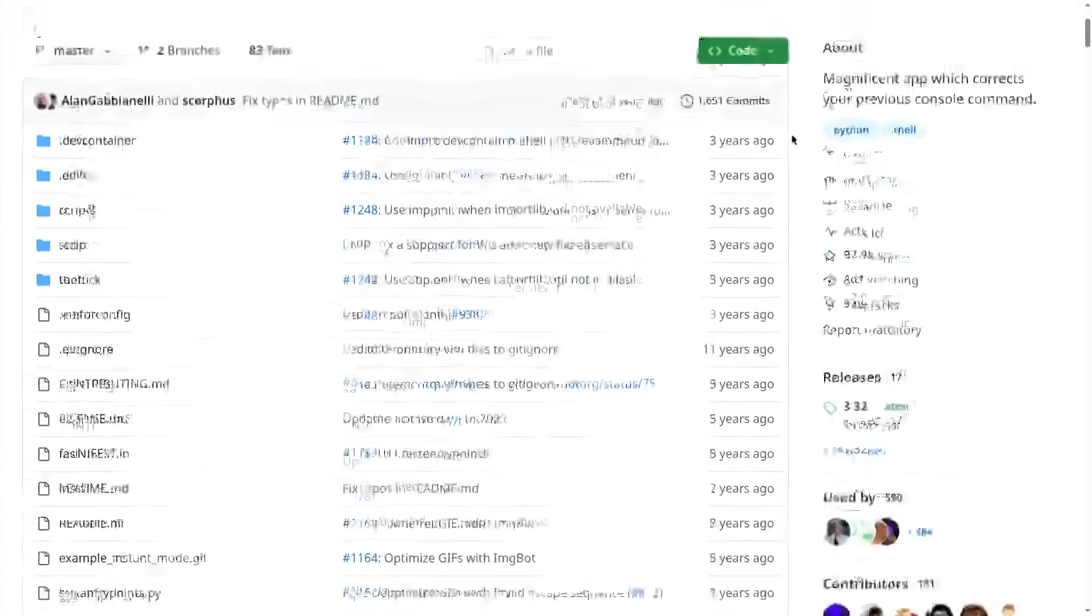
\includegraphics[width=0.92\textwidth]{figures/fig_05_github_thefuck_typo.png}
\caption{GitHub 经典开源项目 \texttt{nvbn/thefuck}：10年前专门用于修正人类程序员在 Shell 命令行中高频手滑 Typo 的工具\vtag}
\end{figure}
\srcnote{00:10:30--00:10:45}

\subsection{经典手滑案例剖析：双层循环把 \texttt{j++} 写成 \texttt{i++}}

为了直观展示“一处微不足道的手滑能引发多么诡异的后果”，我们来看幻灯片第 4 页给出的两行 C 语言双层循环代码（图 6）：

\begin{figure}[H]
\centering
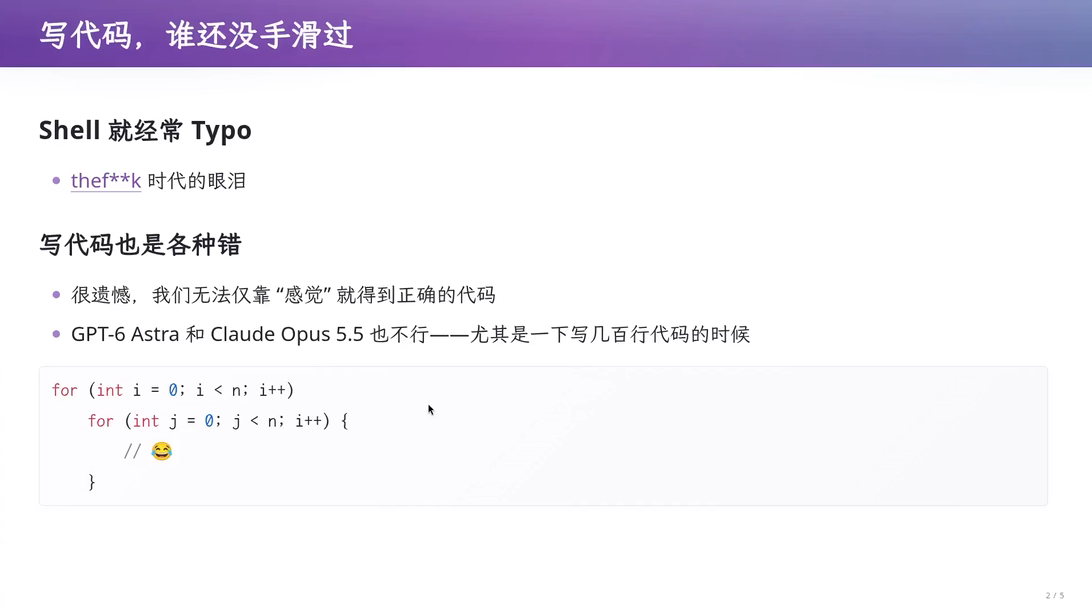
\includegraphics[width=0.92\textwidth]{figures/fig_06_nested_loop_typo_slide.png}
\caption{写代码手滑实例：无论是人类还是 GPT-6 Astra / Claude Opus 5.5，都无法仅靠“感觉”保证几百行代码不出现类似将内层 \texttt{j++} 误写为 \texttt{i++} 的缺陷\vtag}
\end{figure}
\srcnote{00:11:45--00:12:00}

\begin{lstlisting}[language=C, caption={将内层循环步进 \texttt{j++} 误写为 \texttt{i++} 的缺陷代码}]
for (int i = 0; i < n; i++)
    for (int j = 0; j < n; i++) {
        // loop body: do something with (i, j)
    }
\end{lstlisting}

任何参加过算法竞赛或写过矩阵遍历的同学，都曾在深夜写出过上面这段代码：原本想写一个 $n \times n$ 的二维遍历，外层循环变量是 \texttt{i}，内层循环变量是 \texttt{j}；但在写内层 \texttt{for} 的第三个表达式时，由于大脑还停留在外层循环的惯性里，顺手把 \texttt{j++} 敲成了 \texttt{i++}！

这段代码在编译器眼里是\textbf{完全合法的 C 语言程序}，甚至连常规编译警告（Warning）都不会触发。但它在运行时究竟会发生什么？蒋老师在左侧黑板上对这段代码的执行轨迹进行了严密的分类推演（图 7）：

\begin{figure}[H]
\centering
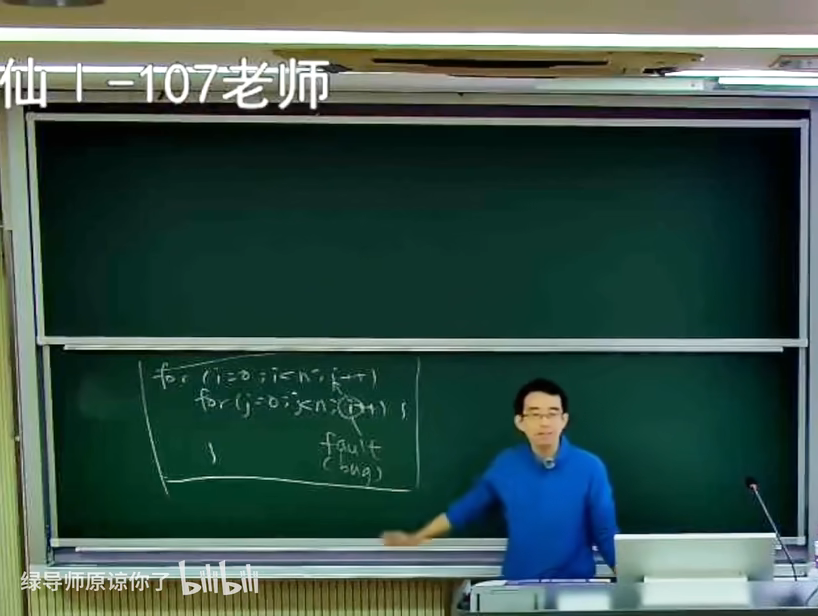
\includegraphics[width=0.92\textwidth]{figures/fig_07_board_nested_loop_ub.png}
\caption{课堂板书：推演双层循环误写 \texttt{i++} 后，当 $n > 0$ 时内层循环条件 $j < n$ 恒成立、导致有符号整数 $i$ 持续自增直至溢出的未定义行为（UB）\vtag}
\end{figure}
\srcnote{00:13:45--00:14:00}

\begin{knowledgebox}{实战推演：双层循环 \texttt{j++} 误写为 \texttt{i++} 的三种运行结局}
假设循环体内部不修改变量 \texttt{i} 和 \texttt{j}，我们按输入参数 $n$ 的取值以及编译优化级别进行分析：
\begin{enumerate}
    \item \textbf{情形一（$n \le 0$）：缺陷被完全掩盖（Fault 未触发 Error）}
    当输入 $n \le 0$（例如空矩阵 $n = 0$）时，外层循环初始条件 \texttt{i = 0; i < n} 在第一次判断时即不成立，程序直接跳过整个双层循环正常返回。此时代码里明明躺着一个 Bug，但外部表现与正确程序 100\% 一致！
    \item \textbf{情形二（$n > 0$，未开启激进优化 \texttt{-O0}）：有符号整数溢出与死循环}
    当 $n \ge 1$ 时，外层循环以 \texttt{i = 0} 进入内层循环，内层初始化 \texttt{j = 0}。由于 $0 < n$ 成立，每次执行完内层循环体后执行的是 \texttt{i++}，而 \textbf{\texttt{j} 的值永远保持为 $0$}！于是内层循环的终止条件 $j < n$（即 $0 < n$）在数学上永远为真。随着内层循环一轮轮空转，外层变量 \texttt{i} 会从 $0, 1, 2, \dots$ 一直加到 32 位有符号整数的最大值 $\text{INT\_MAX} = 2^{31} - 1 = 2,147,483,647$，下一拍再执行 \texttt{i++} 就会发生\textbf{有符号整数溢出（Signed Integer Overflow）}。
    \item \textbf{情形三（$n > 0$，开启现代编译器优化 \texttt{-O2/-O3}）：C 语言未定义行为（UB）引发的诡异穿越}
    在 C 语言标准（ISO C99/C11）中，无符号整数溢出定义为模 $2^w$ 回绕，但\textbf{有符号整数溢出属于未定义行为（Undefined Behavior，UB）}，且无副作用的死循环在特定标准条款下同样涉及 UB。现代编译器（如 GCC/Clang）的优化器会合法地假设“程序中绝不会发生 UB”，从而可能直接把内层循环优化成死锁、或者消掉后续边界检查，产生令程序员目瞪口呆的机器码！
\end{enumerate}
\end{knowledgebox}

这个仅有两个字符之差（\texttt{j} 变成 \texttt{i}）的例子给了我们极其深刻的启示：无论是人类古法编程，还是未来的 GPT-6 Astra 或 Claude Opus 5.5，当一口气生成几百上千行代码时，都绝对无法仅凭“直觉”或“看起来很对”来保证代码没有幻觉。

\begin{warningbox}{常见误区：为什么“编译通过且零 Warning”绝不代表代码没有致命缺陷？}
许多初学者习惯把“编译器不报错”当成代码写对的标志。然而双层循环误写 \texttt{i++} 的案例表明：编译器主要检查语法与静态类型一致性，却无法替你审查控制流步进变量是否匹配业务意图；更危险的是，一旦触发 C/C++ 的有符号整数溢出等未定义行为（UB），优化器甚至会静默改写控制流逻辑。
\end{warningbox}

\subsection{本章小结}

本章通过命令行纠错工具 \texttt{thefuck} 与双层循环误写 \texttt{i++} 的板书推演，揭示了人类与 AI 共享的“编码幻觉”本质：哪怕语法完全合法、甚至在特定输入（如 $n=0$）下表现正常的代码，内部也可能隐藏着触发死循环或未定义行为的致命缺陷。

% =========================================================================
% SECTION 3
% =========================================================================
\section{软件质量的三元模型：Fault、Error 与 Failure}

\subsection{为什么“程序有 Bug”不等于“程序会崩溃”？}

为了把上一节双层循环中观察到的现象上升为严谨的工程理论，软件工程与可信计算（Dependable Computing，如 Avizienis 等人的经典分类体系）将“软件出问题”这一笼统的说法严格拆解为三个处于不同层面的核心概念：**Fault（缺陷）**、**Error（错误状态）**与 **Failure（失效）**（图 8）。

\begin{figure}[H]
\centering
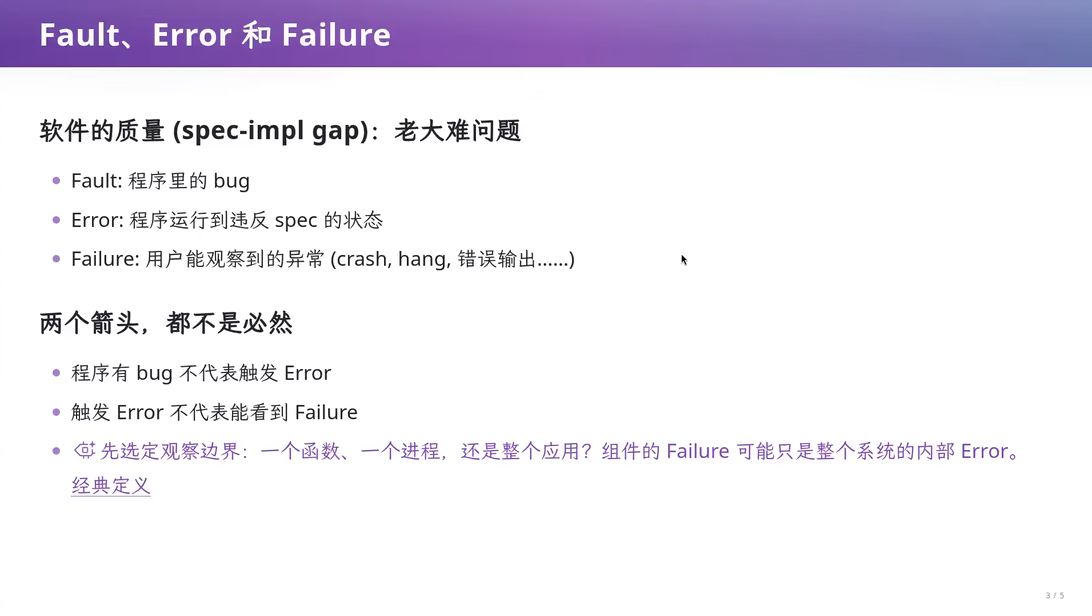
\includegraphics[width=0.92\textwidth]{figures/fig_08_fault_error_failure_slide.png}
\caption{软件质量三元模型：\texttt{Fault}、\texttt{Error} 与 \texttt{Failure} 的严格定义，以及两个非必然转化箭头与观察边界的选择\vtag}
\end{figure}
\srcnote{00:16:00--00:16:15}

蒋老师结合左侧黑板板书（图 9），将软件运行视为状态机在规约空间中的演化轨迹，给出了这三个概念的精确定义：

\begin{figure}[H]
\centering
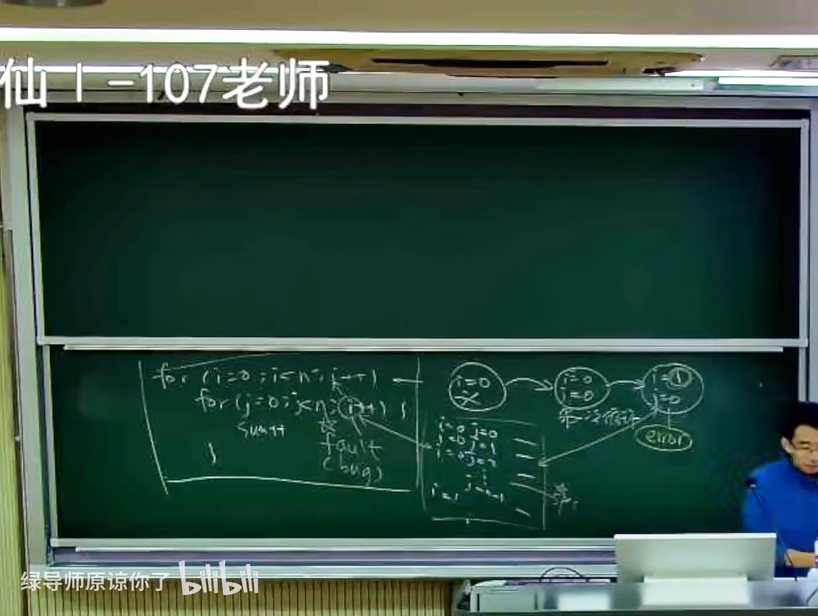
\includegraphics[width=0.92\textwidth]{figures/fig_09_board_fault_error_failure.png}
\caption{课堂板书：静态代码中的 \texttt{Fault} 如何通过特定输入激活为运行时状态偏离 \texttt{Error}，并最终穿透观察边界表现为外部可见的 \texttt{Failure}\vtag}
\end{figure}
\srcnote{00:18:45--00:19:00}

\begin{equation}
\text{Fault（静态缺陷）}
\;\xrightarrow[\text{非必然}]{\;\text{被输入激活}\;}\;
\text{Error（内部脏状态）}
\;\xrightarrow[\text{非必然}]{\;\text{穿透观察边界}\;}\;
\text{Failure（外部失效）}
\end{equation}

上式中三个核心状态及两段跃迁的严格界定如下：
\begin{itemize}
    \item \textbf{\texttt{Fault}（缺陷 / 俗称 Bug）}：存在于程序静态源代码或配置中的瑕疵。它是产生错误的潜在根源，例如把 \texttt{j++} 错写成 \texttt{i++}、漏写了一个分支条件、或者在计算购物车缓存总价时多乘了一个 $2$。只要代码写下了，\texttt{Fault} 就静态地躺在那里，哪怕程序还没被运行。
    \item \textbf{\texttt{Error}（错误状态）}：程序在\textbf{运行过程中（Runtime）}，其内部某个变量、内存数据结构、寄存器或程序计数器的状态偏离了系统规约（Specification）所预期的合法状态集合。例如在双层循环中，第一轮内层迭代结束后原本应当满足 $(i=0, j=1)$，实际运行状态却变成了 $(i=1, j=0)$——此时程序已经进入了 \texttt{Error} 状态。
    \item \textbf{\texttt{Failure}（失效 / 外部异常）}：当内部的 \texttt{Error} 顺着数据流与控制流不断传播，最终穿透了我们选定的\textbf{观察边界（Observation Boundary）}，变成用户或外部调用者能够直接观察到的反常行为——例如程序崩溃（Crash / Segmentation Fault）、死锁卡死（Hang，如原本应该在 0.0001秒内结束的函数迟迟不返回）、或者向用户输出了错误的账单金额。
\end{itemize}

\subsection{两个“非必然”箭头与观察边界的相对性}

理解上式最关键的洞察在于：\textbf{从 Fault 到 Error 的箭头不是必然的，从 Error 到 Failure 的箭头同样不是必然的！}

\begin{table}[H]
\centering
\small
\caption{Fault $\to$ Error $\to$ Failure 传播链中的阻断与演化实例对照表}
\begin{tabular}{p{3.2cm}p{4.8cm}p{5.2cm}}
\toprule
\textbf{传播阶段} & \textbf{为什么该箭头“并非必然”？} & \textbf{具体工程实例} \\
\midrule
\textbf{\texttt{Fault} $\nrightarrow$ \texttt{Error}} & 缺陷所在的静态代码分支未被当前输入执行到，或在当前参数下退化为恒等操作 & 双层循环将 \texttt{j++} 误写为 \texttt{i++}，但测试输入恰好为 $n = 0$；或者 \texttt{add(a,b)} 误写为 \texttt{a - b}，但输入恰好为 $b = 0$ \\
\textbf{\texttt{Error} $\nrightarrow$ \texttt{Failure}} & 内部状态虽然已经算错，但该脏状态从未被后续可见输出读取，或被下游容错逻辑覆盖重写 & 购物车模块更新商品数量时把内部缓存字段 \texttt{cached\_total} 算成了两倍（已触发 \texttt{Error}），但结账接口实际重新遍历商品列表求和而未读取该缓存字段（未造成结账 \texttt{Failure}） \\
\textbf{组件 \texttt{Failure} $=$ 系统 \texttt{Error}} & \textbf{观察边界（Boundary）具有相对性}：局部子系统的外部失效，在更大系统看来可能只是内部的一次异常状态 & 分布式存储中单台节点磁盘写入超时崩溃（对该进程而言已是 \texttt{Failure}），但上层 Raft 共识集群通过多数派副本自动屏蔽了该节点（对整个云服务用户而言仅是一次被消化的内部 \texttt{Error}） \\
\bottomrule
\end{tabular}
\end{table}

此外，蒋老师特别强调了**非功能性规约（Non-functional Spec）下的 Failure 判定**：如果一个函数的规约要求不仅计算结果正确，还必须在规定时间内响应（例如正常情况下 0.0001秒就应该执行完毕），那么当程序因为误写 \texttt{i++} 而陷入长达数秒的空转或卡死时，“迟迟不返回”本身就已经构成了用户可观测的 \texttt{Failure}。

\begin{importantbox}{核心辨析：观察边界（Observation Boundary）如何决定 Error 与 Failure 的转化}
在讨论 \texttt{Error} 与 \texttt{Failure} 时，第一步永远是**先画定观察边界**：
\begin{itemize}
    \item 若以**单个函数**为边界，返回值算错 $1$ 比特就是该函数的 \texttt{Failure}；
    \item 若以**整个应用程序或分布式集群**为边界，单个子函数或单台节点的 \texttt{Failure} 只要被外层重试、主备切换或容错逻辑成功掩盖，它就退化成了整个大系统内部被消化的一次 \texttt{Error}，不会演变为面向最终用户的系统级 \texttt{Failure}。
\end{itemize}
\end{importantbox}

\subsection{历史警钟：1996 年阿丽亚娜 5 号（Ariane 501）火箭解体事故}

为了说明 Fault、Error 与 Failure 链条在真实工程系统中是如何一步步演变成世纪灾难的，同时揭示“观察边界与冗余备份”的深刻教训，我们来看幻灯片第 6 页详述的软件工程史上最著名的事故之一——**1996 年 6 月 4 日欧洲航天局阿丽亚娜 5 号（Ariane 5 Flight 501）运载火箭首飞解体事故**（图 10）。

\begin{figure}[H]
\centering
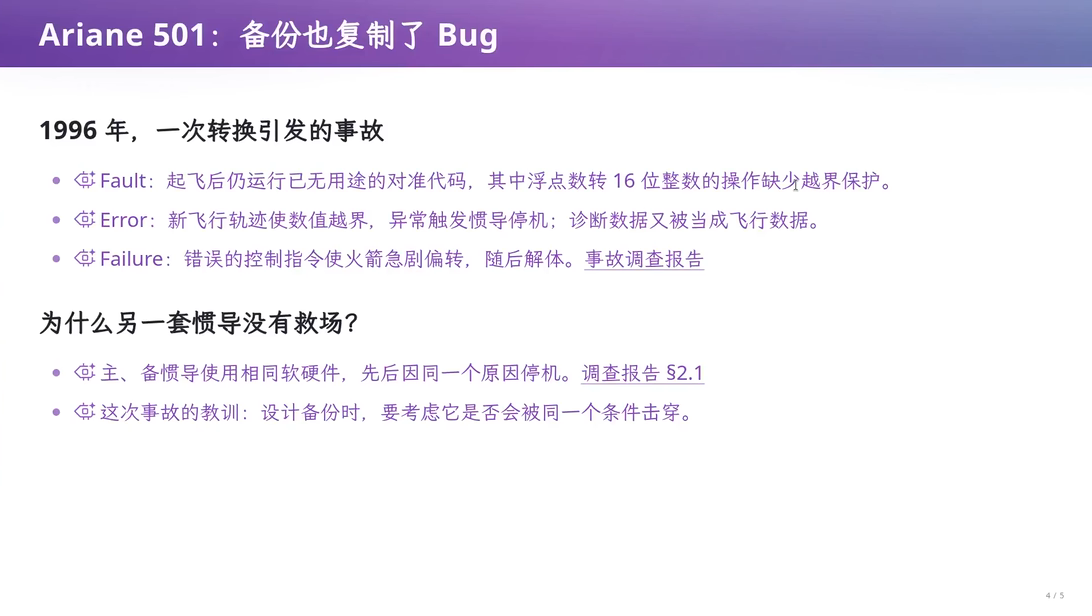
\includegraphics[width=0.92\textwidth]{figures/fig_10_ariane_501_disaster.png}
\caption{Ariane 501 火箭事故剖析：64 位浮点数转 16位整数越界引发惯导停机，且主、备惯导因复制完全相同的软硬件而先后因同一条件击穿\vtag}
\end{figure}
\srcnote{00:22:15--00:22:30}

阿丽亚娜 5 号耗资数十亿美元、研发历时 10年，却在首飞点火升空仅约 37 秒后突然剧烈偏航并触发自毁解体。事后事故调查委员会（Lions Report，§2.1）还原出的完整因果链，堪称 \texttt{Fault $\to$ Error $\to$ Failure} 教科书级的范本：

\begin{warningbox}{经典事故复盘：Ariane 501 是如何被一行类型转换代码摧毁的？}
\begin{enumerate}
    \item \textbf{潜伏的静态缺陷（Fault）——复用旧代码且缺少越界保护}：
    阿丽亚娜 5 号的惯性参考系统（SRI，即惯导模块）直接复用了前代阿丽亚娜 4 号（Ariane 4）的代码。其中有一段负责在发射前校准对准（Alignment）的后台任务，设计为点火起飞后继续运行约 40 秒（这一设计对 Ariane 4 的发射流程有意义，但对 Ariane 5 起飞后其实已毫无用途）。在这段代码里，有一行将与火箭水平速度相关的 \textbf{64 位浮点数转换为 16位有符号整数}（取值范围 $[-32768, +32767]$）的指令，且当年为了节省处理器开销，工程师在分析 Ariane 4 的轨迹上限后认为该变量绝不会越界，因此**没有为这次转换编写越界异常处理保护**。
    \item \textbf{激活内部错误状态（Fault $\to$ Error）——新火箭推力更大导致数值越界}：
    阿丽亚娜 5 号的推力与起飞加速度远大于阿丽亚娜 4 号。升空约 37 秒后，水平速度关联的 64 位浮点数值超过了 $32767$，在转换为 16位有符号整数时瞬间触发硬件算术溢出异常（Operand Error）！
    \item \textbf{主备冗余同时击穿（共模失效 Common-Mode Failure）}：
    火箭设计师当然考虑到了硬件故障的可能性，专门配置了**主惯导（Active SRI）与备份惯导（Backup SRI）双机热备**。然而，主惯导和备份惯导运行的是**完全相同的软件代码、接收完全相同的飞行姿态传感器输入**！结果，备份惯导在主惯导溢出停机的前一个毫秒（约 0.05 秒内），就已经因为一模一样的 16位整数越界而先行崩溃停机了！
    \item \textbf{跨边界传播为灾难性失效（Error $\to$ Failure）——诊断数据被当成飞行姿态}：
    当主惯导也因未捕获异常而按预设嵌入式策略停机时，它向火箭主飞控计算机（OBC）的总线发送了一串用于事后调试的 **诊断位模式（Diagnostic Bit Pattern，即报错码）**。然而飞控计算机并未正确识别惯导已下线，而是把这串报错诊断数据当成了真实的飞行偏航角度数据！飞控计算机误以为火箭发生了极端偏转，立即指令助推器与主发动机喷管打到最大偏转角；猛烈的气动负载瞬间撕裂箭体，触发火箭自毁系统。
\end{enumerate}
\end{warningbox}

Ariane 501 事故给所有系统架构师留下了三条血泪教训：
\begin{itemize}
    \item \textbf{规约随环境演化而失效}：在 Ariane 4 环境里“永远不会超过 16位整数上限”的隐式假设，移植到 Ariane 5 的新物理轨迹下就变成了致命的 \texttt{Fault}；
    \item \textbf{组件级错误处理策略必须对齐全系统目标}：对于地面测试软件，“遇到异常立即 Dump 错误码并停机”是极佳的调试策略；但对于正在万米高空飞行的火箭惯导，“因为一个起飞后根本用不着的校准变量溢出就把整个导航系统关停”，是彻底颠倒了局部与全局的优先级；
    \item \textbf{同构备份防不住软件 Bug}：硬件随机老化故障通常是统计独立的，因此两套相同硬件可以降低故障率；但**软件是确定性的逻辑过程**——如果主节点和备份节点运行同一份代码并面对同一个触发输入，它们会在同一时刻被同一个条件 100\% 击穿！
\end{itemize}

\subsection{本章小结}

本章建立了 \texttt{Fault（静态缺陷） $\to$ Error（内部脏状态） $\to$ Failure（外部可见失效）} 三元模型，阐明了两条转化箭头的非必然性与观察边界的相对性，并通过 1996 年 Ariane 501 火箭 16位整数溢出事故揭示了规约迁移与同构备份的工程陷阱。

% =========================================================================
% SECTION 4
% =========================================================================
\section{质量保障的基本方法：测试与断言的双轮驱动}

\subsection{预防防线：更好的架构与不容易伤人的编程语言}

既然软件缺陷如此危险，我们在工程上有哪些基本武器来保障质量？幻灯片第 7 页（图 11）首先指出了最前置的预防防线：**选择更好的系统架构、使用“不容易伤人”的现代编程语言，以及坚持防御性编程（Defensive Programming）**。

\begin{figure}[H]
\centering
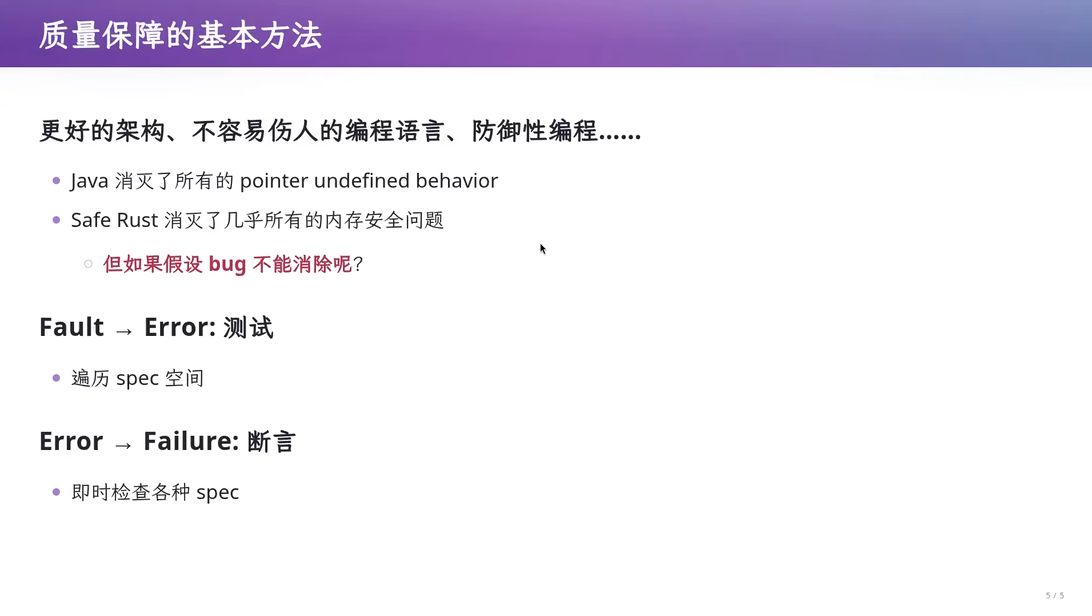
\includegraphics[width=0.92\textwidth]{figures/fig_11_qa_basic_methods_slide.png}
\caption{质量保障的基本方法：通过 Java / Safe Rust 消除底层未定义行为，并利用测试（\texttt{Fault $\to$ Error}）与断言（\texttt{Error $\to$ Failure}）双轮驱动暴露残余缺陷\vtag}
\end{figure}
\srcnote{00:25:45--00:26:00}

编程语言的演进史，本质上就是把原本需要程序员人肉遵守的隐式规约（Spec），一步步收编为编译器与运行时强制执行的静态/动态检查史：
\begin{itemize}
    \item \textbf{Java 彻底消灭了指针未定义行为（Pointer Undefined Behavior）}：在 C 语言中，你可以把任意整数（如 \texttt{0x12345678}）强制类型转换为指针并解引用，或者发生数组越界覆盖相邻栈帧而不报错；而在 Java 中，没有任意指针算术，任何空引用解引用或数组越界都会由 JVM 确定性地抛出 \texttt{NullPointerException} 或 \texttt{ArrayIndexOutOfBoundsException}，绝不会静默破坏内存。
    \item \textbf{Safe Rust 在编译期消灭了几乎所有内存安全与数据竞争问题}：通过所有权（Ownership）、借用检查器（Borrow Checker）与生命周期（Lifetime）类型系统，Safe Rust 将悬垂指针（Dangling Pointer）、二次释放（Double Free）以及并发读写冲突直接拦截在编译阶段。
\end{itemize}

课堂上，蒋老师还在左侧黑板（图 13）上剖析了为什么 C 语言系统编程如此考验功力：当你调用 \texttt{malloc} 分配一块内存后，规约要求在所有退出路径上都必须配对调用 \texttt{free}；然而函数中往往存在多条提前 \texttt{return} 的异常分支，甚至可能存在跨函数的 \texttt{setjmp / longjmp} 非局部跳转。正因如此，Linux 内核代码才演化出了著名的 \texttt{goto out\_free;} 集中式资源释放编码规范，用结构化的编程纪律来降低人类手滑漏写 \texttt{free} 的概率。

\subsection{当 Bug 无法彻底消除时：测试与断言的正交分工}

然而，即便使用了 Safe Rust 或 Java，业务层面的逻辑 Bug（例如把加法写成减法、把选课名额上限判错、把火箭校准代码留在起飞后运行）依然无法靠编译器自动消除。**如果我们诚实地假设“程序里一定还有残留的 Bug（Fault）”，那么质量保障的核心任务就变成了：如何在软件交付给真实用户之前，尽可能把隐藏的 Fault 揪出来？**

蒋老师在左侧黑板上绘制了一幅极具启发性的**程序状态空间几何图景**（图 12），将质量保障的两大核心手段——**测试（Testing）**与**断言（Assertion）**——统一到了上式的两个箭头之上：

\begin{figure}[H]
\centering
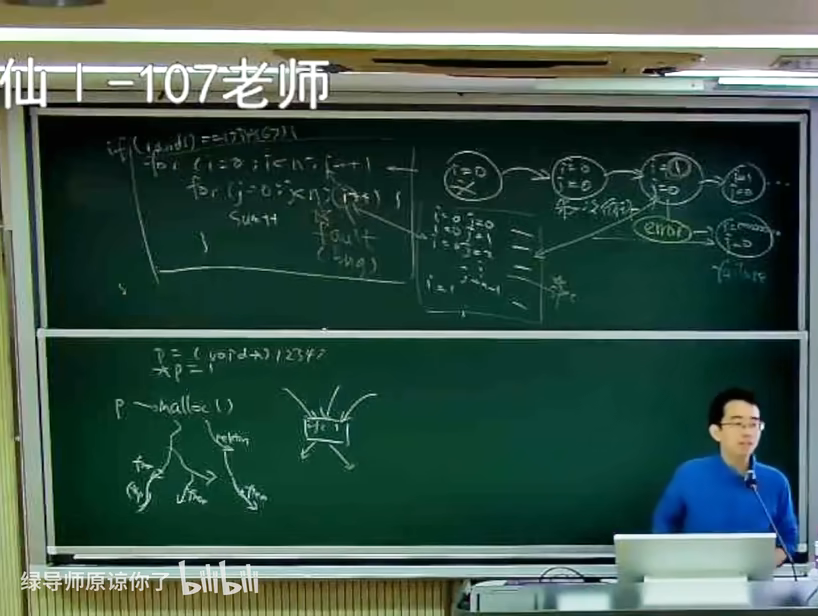
\includegraphics[width=0.92\textwidth]{figures/fig_12_board_state_space_qa.png}
\caption{课堂板书：在程序运行状态空间中，测试（Testing）负责寻找触发路径将 \texttt{Fault} 转化为 \texttt{Error}，断言（Assertion）负责在内部设立哨卡将 \texttt{Error} 即时转化为 \texttt{Failure}\vtag}
\end{figure}
\srcnote{00:29:15--00:29:30}

\begin{figure}[H]
\centering
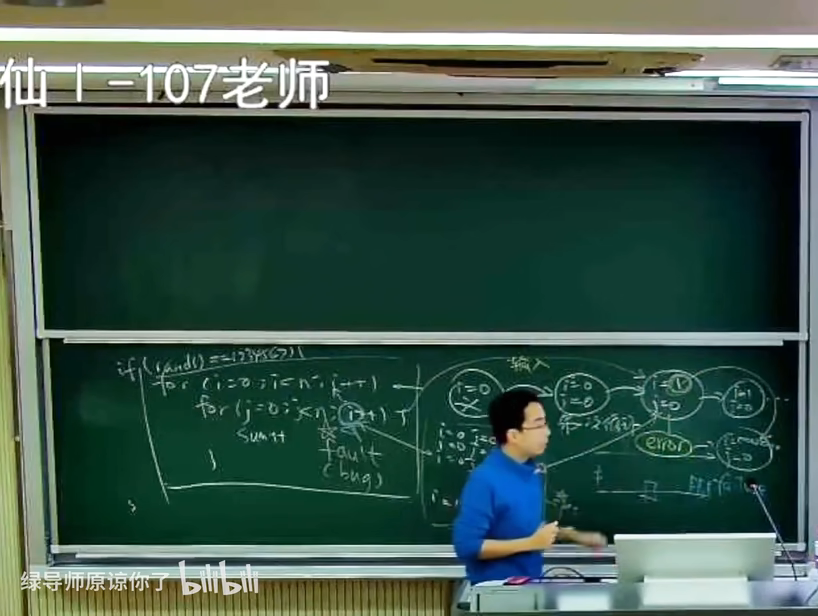
\includegraphics[width=0.92\textwidth]{figures/fig_13_board_pointer_malloc_spec.png}
\caption{课堂板书：C 语言指针解引用、\texttt{malloc/free} 生命周期配对、提前 \texttt{return/longjmp} 异常控制流与 Linux \texttt{goto} 错误清理范式\vtag}
\end{figure}
\srcnote{00:34:15--00:34:30}

让我们用形式化的集合语言来刻画这一双轮驱动机制。设程序的广义输入空间为 $\mathcal{I}$，程序在输入 $x \in \mathcal{I}$ 下的执行轨迹为状态序列 $\tau(x) = \langle s_0, s_1, \dots, s_T \rangle$，规约所允许的合法内部状态集合为 $\mathcal{S}_{\mathrm{spec}}$，而在系统最外层观察边界上可被检测到的异常状态集合为 $\mathcal{S}_{\mathrm{obs\_fail}}$。由于在没有内部检查的情况下，偏离规约的错误状态集合 $\mathcal{S}_{\mathrm{error}} = \mathcal{S} \setminus \mathcal{S}_{\mathrm{spec}}$ 往往远大于最终暴露给外部的失效集合（即很多内部 \texttt{Error} 被静默吞掉或延迟了很久才爆发），我们引入运行时断言谓词族 $\{P_k(s)\}_{k=1}^m$，从而构成如下正交协同关系：

\begin{equation}
\begin{cases}
\textbf{Testing}: & \text{搜索 } x \in \mathcal{I}_{\mathrm{test}}, \;\text{使 } \exists\, t,\; s_t(x) \in \mathcal{S}_{\mathrm{error}} \quad (\mathtt{Fault \to Error}) \\[6pt]
\textbf{Assertion}: & \text{注入 } \mathtt{assert}(P_k(s_t)), \;\text{当 } s_t \in \mathcal{S}_{\mathrm{error}} \text{ 时触发异常} \quad (\mathtt{Error \to Failure})
\end{cases}
\end{equation}

上式揭示了为什么**没有断言配合的测试是事倍功半的，而没有测试驱动的断言是孤掌难鸣的**：
\begin{enumerate}
    \item \textbf{测试的职责（\texttt{Fault $\to$ Error}）：遍历规约输入空间}
    静态代码里的 \texttt{Fault} 就像埋在地下的地雷。测试（Testing）的本质，就是构造各种各样的输入与运行环境，像扫雷车一样尽可能走遍代码的不同分支与状态组合，争取踩中那颗地雷，让程序内部进入错误的 \texttt{Error} 状态。
    \item \textbf{断言的职责（\texttt{Error $\to$ Failure}）：压缩错误潜伏期，即时拉响警报}
    如果程序踩中了地雷（进入了 \texttt{Error} 状态），但内部没有任何检查，这个脏状态可能还会静默运行几千万条指令（就像双层循环 \texttt{i++} 空转几十亿次，或者像《仙剑奇侠传》在模拟器里跑飞前已经悄悄算错了一个寄存器），直到很久以后才在毫不相干的地方崩溃，甚至干脆没有引起外部可见崩溃而被漏掉。**断言（\texttt{assert}）的作用，就是在程序内部的关键关节处密集布置传感器，把观察边界直接前移到代码内部**！一旦某个不变量（如 \texttt{assert(j > prev\_j)} 或数据结构完整性检查）被违反，当场就在第一案发现场触发 \texttt{Failure} 报错停机，既防止了 \texttt{Error} 被静默掩盖，又省去了顺着漫长调用链反向追查根因的痛苦。
\end{enumerate}

\subsection{本章小结}

本章阐明了软件质量保障的双轮驱动模型：一方面通过内存安全语言（Java / Safe Rust）和防御性编程减少 \texttt{Fault} 的引入；另一方面在假设 \texttt{Fault} 必然残留的前提下，依靠**测试（遍历规约空间，促成 \texttt{Fault $\to$ Error}）**与**断言（即时检查规约不变量，促成 \texttt{Error $\to$ Failure}）**的正交配合，让隐藏的错误无处遁形。

\begin{knowledgebox}{对比总结：Testing（测试）与 Assertion（断言）在状态空间中的正交职责}
\begin{itemize}
    \item \textbf{只有测试、没有内部断言}：即使测试输入踩中了 \texttt{Fault} 并触发了内部 \texttt{Error}，脏状态也可能被下游逻辑偶然掩盖，或跑出数千万条指令后才在远端崩溃，导致漏检或极难定位根因；
    \item \textbf{只有内部断言、没有充分测试}：断言哨卡虽然立在代码里，但如果测试输入过于单一、从未走到缺陷分支（\texttt{Fault $\nrightarrow$ Error}），断言就永远不会被触发；
    \item \textbf{测试 $+$ 断言双剑合璧}：用高覆盖、高区分度的测试主动把系统逼入边界状态，再用密集的运行时 \texttt{assert} 在错误发生的第一现场立即引爆 \texttt{Failure}！
\end{itemize}
\end{knowledgebox}

% =========================================================================
% SECTION 5
% =========================================================================
\section{“在我机器上能跑”说明了什么：广义输入空间与 Agent 反馈闭环}

\subsection{为什么“顺便运行几次”远没那么简单？——环境与 \texttt{package-lock.json}}

从表面上看，测试似乎是世界上最“便宜”的质量保障方法——代码写完了，顺便在终端里运行几次看看结果对不对呗！哪怕运行 1次不够放心，那我连续运行 100次、1000次，甚至运行 1万次的时候都没报错，总该说明程序没问题了吧？

幻灯片第 8 页（图 14）直截了当地打破了这种天真幻想：**“在你的机器上能跑”，往往只说明了它在你当前这台机器、当前这一秒钟、当前这组特定配置下碰巧没炸而已！**

\begin{figure}[H]
\centering
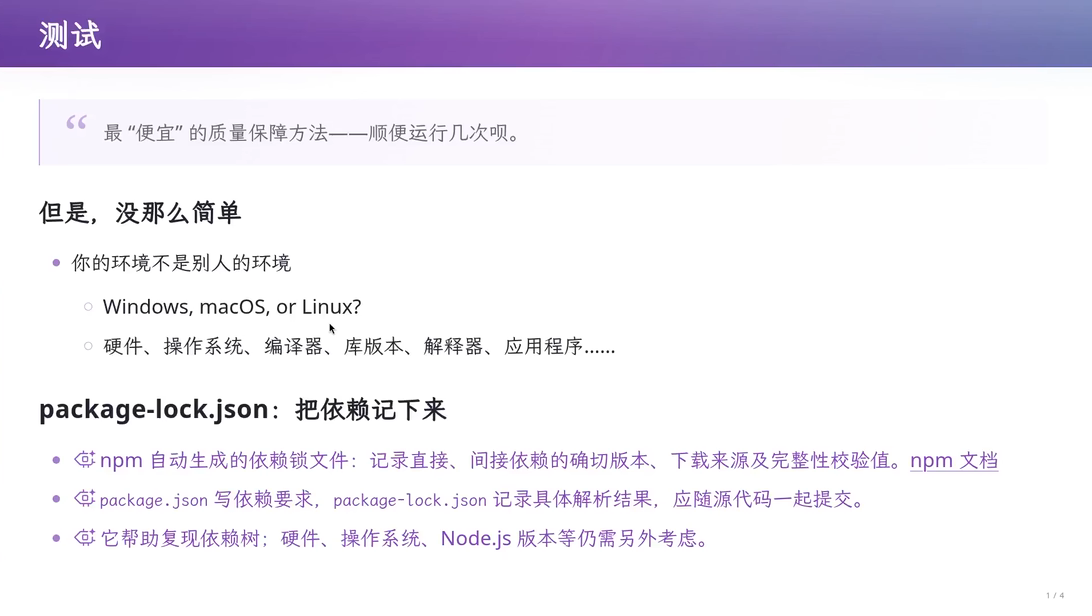
\includegraphics[width=0.92\textwidth]{figures/fig_14_testing_env_package_lock.png}
\caption{测试并非只是“顺便运行几次”：跨平台环境差异（Windows/macOS/Linux、内核、编译器、库版本）与 \texttt{package-lock.json} 依赖锁文件的能力边界\vtag}
\end{figure}
\srcnote{00:37:45--00:38:00}

蒋老师结合左侧黑板板书（图 15），剖析了为什么“你的环境不是别人的环境”：
\begin{enumerate}
    \item \textbf{底层软硬件栈的巨大分异}：
    你的程序运行在 macOS（ARM64 架构）、Windows 还是 Linux（x86\_64 架构）上？不同架构下的字节序、内存序（Memory Ordering，如 ARM 的弱内存模型 vs x86 的 TSO 强内存模型）、页面大小（4 KB vs 16 KB）、操作系统内核版本、C 标准库（\texttt{glibc} vs \texttt{musl}）、编译器版本乃至 Python/Node.js 解释器的小版本差异，都可能让同一份源代码展现出截然不同的行为。
    \item \textbf{\texttt{package.json} 与 \texttt{package-lock.json} 的工程分工与局限}：
    在现代前端与 Node.js 工程中，开发者在 \texttt{package.json} 里编写的往往是带有语义化版本范围的依赖声明（例如 \texttt{"lodash": "\^{}4.17.0"}）。如果只提交 \texttt{package.json}，那么你的同事或生产服务器在明天执行 \texttt{npm install} 时，解析到的直接依赖或深层间接依赖（Transitive Dependencies）版本就可能已经悄悄升级，从而引入破坏性变更。
    为此，\texttt{npm} 引入了自动生成的锁文件 \textbf{\texttt{package-lock.json}}：它精确记录了整棵依赖树上每一个直接与间接依赖包的**确切版本号、下载源 URL 以及密码学完整性校验哈希值（Integrity Hash）**，因此必须随源代码一起提交到 Git 仓库中。但即便锁死了 \texttt{package-lock.json}，它也只能复现应用层依赖树——底层的硬件架构、操作系统内核与 Node.js 运行时版本依然在它的锁定范围之外。
\end{enumerate}

\begin{figure}[H]
\centering
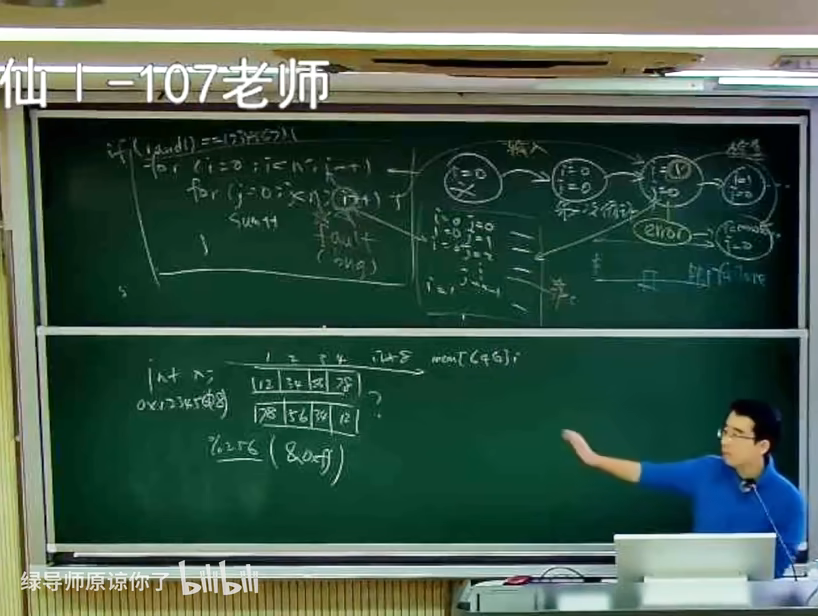
\includegraphics[width=0.92\textwidth]{figures/fig_15_board_environment_inputs.png}
\caption{课堂板书：程序的真实输入不仅包含显式函数参数，还包含底层操作系统、动态库与运行时环境等隐式维度\vtag}
\end{figure}
\srcnote{00:41:45--00:42:00}

\subsection{同一份程序，不同的运行：时间、负载与并发线程调度交错}

更进一步，即便在同一台物理机器、同一个 Docker 容器镜像里，用完全相同的命令行参数把同一份二进制程序运行两遍，它的执行轨迹就一定相同吗？幻灯片第 9 页（图 16）给出了否定的回答：**同一份程序，每次运行面对的“隐式输入”都在剧烈变化！**

\begin{figure}[H]
\centering
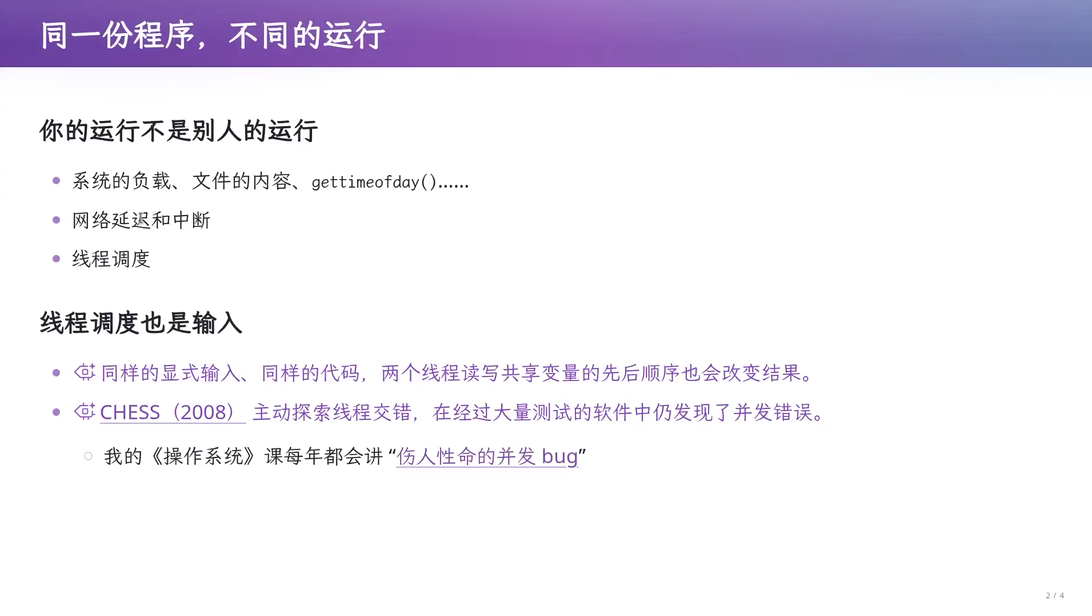
\includegraphics[width=0.92\textwidth]{figures/fig_16_nondeterministic_runs_chess.png}
\caption{同一份程序的不同运行：系统负载、文件内容、\texttt{gettimeofday()}、网络延迟中断，以及 CHESS（2008）主动探索的并发线程调度交错，全都是程序的广义输入\vtag}
\end{figure}
\srcnote{00:44:00--00:44:15}

如果我们从操作系统与体系结构的视角审视一个进程（Process），所谓“输入”绝非只有 \texttt{main(int argc, char *argv[])} 里的参数，而是**所有从进程外部流入进程状态空间的比特信息总和**：

\begin{equation}
\mathcal{I}_{\mathrm{total}}
= \mathcal{I}_{\mathrm{explicit}} \;\times\; \mathcal{I}_{\mathrm{env}} \;\times\; \mathcal{I}_{\mathrm{clock}} \;\times\; \mathcal{I}_{\mathrm{net/disk}} \;\times\; \mathcal{I}_{\mathrm{sched}}
\end{equation}

上式中五个正交分量揭示了为什么许多棘手的 Bug 具有“海森堡 Bug（Heisenbug）”般的偶发性：
\begin{itemize}
    \item $\mathcal{I}_{\mathrm{explicit}}$（显式参数与标准输入）：命令行参数、函数调用实参、标准输入流；
    \item $\mathcal{I}_{\mathrm{env}}$（环境与文件系统状态）：环境变量、当前工作目录、磁盘文件内容、可用内存与 CPU 负载；
    \item $\mathcal{I}_{\mathrm{clock}}$（系统时钟与定时器）：程序每次调用 \texttt{gettimeofday()} 或 \texttt{clock\_gettime()} 读到的时间戳都不同。正如课堂所举的例子：假设当前时刻为 $T$，程序在 $T + 1\text{秒}$ 的时刻执行某分支，或者在 $T + 1\text{毫秒}$ 的时刻恰好跨越了整秒/整天边界（甚至闰秒、时间戳回拨），就可能触发平日运行 1万次都遇不到的时间戳拼接或缓存过期 Bug；
    \item $\mathcal{I}_{\mathrm{net/disk}}$（I/O 延迟与中断）：网络数据包是分两次 \texttt{read()} 到达还是一次到达？磁盘写入中途是否发生超时或信号中断（\texttt{EINTR}）？
    \item $\mathcal{I}_{\mathrm{sched}}$（多线程调度交错，Thread Interleaving）：这是系统软件中最隐蔽、最致命的输入源！当两个线程并发读写共享变量时，哪怕显式输入完全固定，操作系统调度器在哪一条机器指令边界上切换线程，也会彻底改变执行结果。
\end{itemize}

为了直观说明并发调度交错如何制造隐藏的 \texttt{Error}，我们来看一个最简单的多线程共享计数器更新：

\begin{lstlisting}[language=C, caption={并发线程读写共享变量导致更新丢失（Lost Update）的指令级交错}]
// Shared state: int counter = 0;
// Both Thread A and Thread B execute: counter = counter + 1;
// Machine-level decomposition of (counter = counter + 1):
//   R1 = LOAD(counter)
//   R1 = R1 + 1
//   STORE(counter, R1)

// Normal sequential execution (counter becomes 2):
//   Thread A: LOAD(0) -> ADD(1) -> STORE(1)
//   Thread B:                               LOAD(1) -> ADD(2) -> STORE(2)

// Interleaved execution under preemption (counter becomes 1 -> ERROR!):
//   Thread A: LOAD(0) -> ADD(1) ... [Context Switch] ...          -> STORE(1)
//   Thread B:                       LOAD(0) -> ADD(1) -> STORE(1)
\end{lstlisting}

在上面的交错中，线程 A 刚刚把 \texttt{counter = 0} 读入寄存器并加 $1$，还没来得及写回内存，操作系统时钟中断恰好到来并切换到线程 B；线程 B 读到的依然是旧值 $0$，加 $1$ 后写回 $1$；随后线程 A 恢复执行，把寄存器里的 $1$ 写回内存——**两次自增操作全部成功执行完毕，没有任何崩溃，但最终结果却从规约预期的 $2$ 变成了错误的 $1$！**

在常规测试中，由于一条加法指令耗时仅纳秒级，时钟中断恰好卡在 \texttt{LOAD} 与 \texttt{STORE} 之间的概率极低，你可能在本地连续跑 1000次、1万次都全部通过；但一旦上线到高并发生产环境，这种错误每天都会批量发生，甚至造成灾难性的后果。蒋老师在课堂上专门展示了他在《操作系统》课上每年必讲的经典视频《伤人性命的并发 Bug》（图 17，讲述了 Therac-25 放射治疗仪因并发竞态条件导致患者接受过量辐射致死、以及北美大停电等真实历史惨剧），并介绍了微软研究院开发的并发测试工具 **CHESS（2008）**：CHESS 通过接管线程调度器，用系统化的状态空间搜索主动枚举不同的线程交错顺序，在已经通过了海量常规测试的工业级并发软件中依然揪出了大量潜伏的并发缺陷。

\begin{figure}[H]
\centering

\includegraphics[width=0.92\textwidth]{figures/fig_17_concurrency_bug_video.png}
\caption{《操作系统》课程关联回顾：“伤人性命的并发 Bug”——线程调度交错不仅是程序的隐式输入，更曾在真实工业史上酿成惨重事故\vtag}
\end{figure}
\srcnote{00:45:00--00:45:15}

\subsection{程序的正确性、Dijkstra 名言与 $1/n!$ 的数学信心}

既然程序的广义输入空间 $\mathcal{I}_{\mathrm{total}}$ 如此庞大，我们该如何定义“程序的正确性（Program Correctness）”？幻灯片第 10 页（图 18）给出了完整定义：

\begin{figure}[H]
\centering
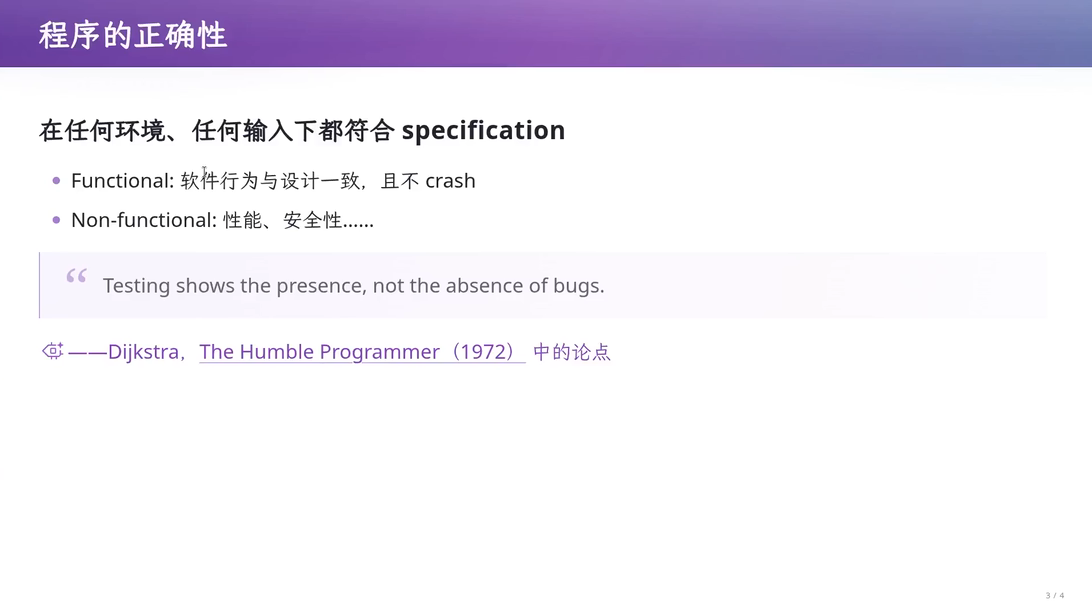
\includegraphics[width=0.92\textwidth]{figures/fig_18_program_correctness_dijkstra.png}
\caption{程序的正确性：在任何环境、任何输入下均满足功能性（Functional）与非功能性（Non-functional）规约，以及 Dijkstra（1972）的著名论断\vtag}
\end{figure}
\srcnote{00:46:00--00:46:15}

一个真正正确的程序，必须在**任何目标环境、任何合法输入（含恶劣外部输入）**下同时满足两类规约：
\begin{enumerate}
    \item \textbf{功能性规约（Functional Specification）}：软件的计算结果与状态演化和设计文档严格一致，且绝不发生非预期崩溃（Crash）或死锁；
    \item \textbf{非功能性规约（Non-functional Specification）}：包括**性能（Performance）**（如高负载下尾延迟不超标、算法复杂度不退化）与**安全性（Security）**（如未登录或低权限用户绝不能通过构造恶意请求越权查看或篡改他人数据）。
\end{enumerate}

面对如此严苛的全称量词要求（$\forall\, x \in \mathcal{I}_{\mathrm{total}},\; \mathrm{Impl}(x) \models \mathrm{Spec}(x)$），图灵奖得主 Edsger W. Dijkstra 在其 1972 年图灵奖演讲《The Humble Programmer》中留下了一句流传半个世纪的名言：

\begin{quote}
\textit{``Program testing can be a very effective way to show the presence of bugs, but it is hopelessly inadequate for showing their absence.''}\\
——**“程序测试能非常有效地显示 Bug 的存在，却绝无可能证明 Bug 的不存在。”**（Edsger W. Dijkstra, 1972）
\end{quote}

既然有限次测试永远无法穷尽无穷的输入空间、无法在数学上证明“绝对没有 Bug”，那为什么工业界还要花如此巨大的精力去写测试？幻灯片第 11 页（图 19）与左侧黑板板书（图 20）从数学概率与智能体反馈两个角度给出了极具说服力的解答：

\begin{figure}[H]
\centering
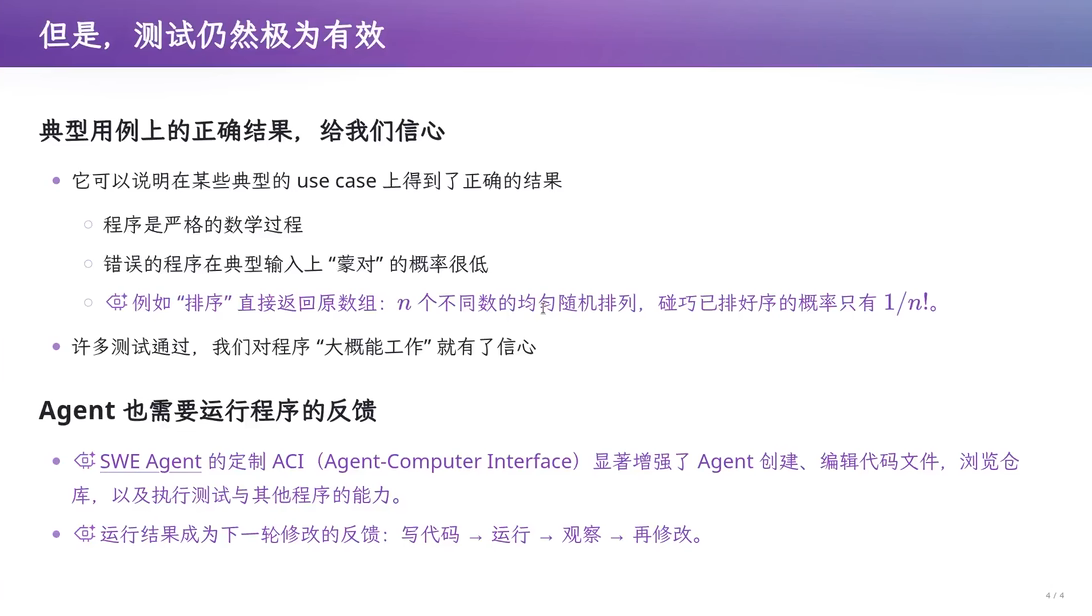
\includegraphics[width=0.92\textwidth]{figures/fig_19_testing_effectiveness_swe_agent.png}
\caption{测试为何仍然极为有效：程序是严格的数学过程，错误程序在典型随机用例上“蒙对”的概率极低（如伪排序函数仅为 $1/n!$），且测试运行构成了 Agent 的核心反馈闭环\vtag}
\end{figure}
\srcnote{00:48:30--00:48:45}

\begin{figure}[H]
\centering
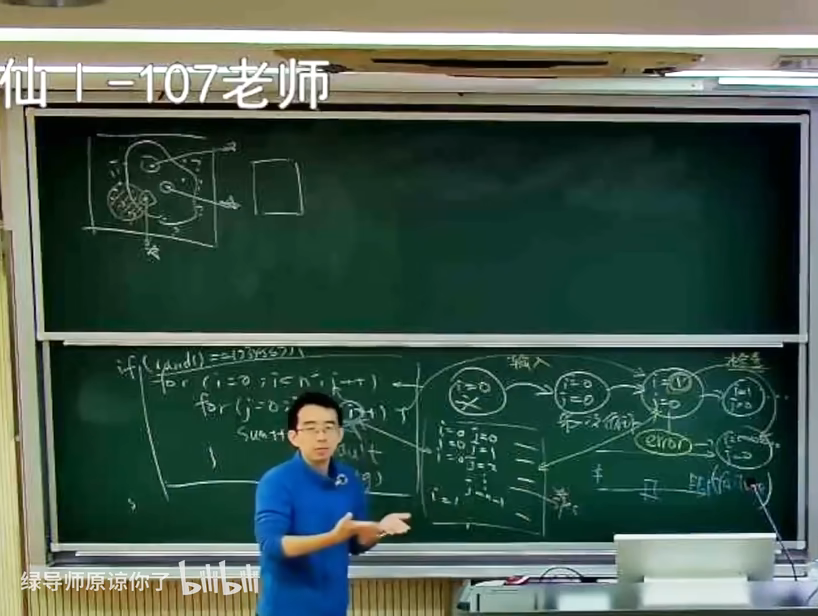
\includegraphics[width=0.92\textwidth]{figures/fig_20_board_spec_sampling_loop.png}
\caption{课堂板书：在规约输入空间中通过测试采样建立概率信心，并构建“写代码 $\to$ 运行 $\to$ 观察 $\to$ 再修改”的闭环\vtag}
\end{figure}
\srcnote{00:51:15--00:51:30}

\textbf{第一，程序是高度敏感的严格数学过程，错误的程序在有区分力的典型输入上“碰巧蒙对”的概率呈阶乘或指数级衰减。}
想象一个极端的例子：某个偷懒的程序员（或产生幻觉的 Agent）写了一个错误的排序函数 \texttt{bad\_sort(arr)}，它内部什么都没干，直接把原数组原封不动地返回了。如果我们只测空数组 \texttt{[]}、单元素数组 \texttt{[1]} 或已经排好序的数组 \texttt{[1, 2, 3]}，这个伪排序函数确实能“蒙混过关”。但只要我们在测试中加入一个包含 $n$ 个互不相同元素的均匀随机排列数组，由于 $n$ 个不同元素共有 $n!$ 种等可能的排列方式，而其中严格递增的正确排列只有唯一 $1$ 种，因此该错误实现碰巧返回正确结果的概率为：

\begin{equation}
\Pr\big[\mathtt{bad\_sort}(\pi) = \mathrm{sorted}(\pi)\big]
= \frac{1}{n!}
\;\xrightarrow{\;n = 10\;}\;
\frac{1}{3,628,800} \approx 2.76 \times 10^{-7}
\end{equation}

其中 $\pi$ 表示从 $n$ 元对称群 $S_n$ 中均匀随机抽取的一个排列。由上式可见，哪怕仅仅取 $n = 10$，一个什么都不干的伪排序函数在单次随机测试中碰巧蒙对的概率就只有三百六十万分之一；如果取 $n = 20$，这个概率更是低至 $1/20! \approx 4.1 \times 10^{-19}$！换句话说，虽然测试不能提供 $100\%$ 的形式化数学证明，但只要我们的测试用例覆盖了系统的典型主路径与随机扰动，随着独立测试用例子弹越打越多，我们对“这个软件在绝大多数常规工况下大概能正常工作”的工程信心就会迅速逼近 $1$。

\subsection{Agent 也需要运行程序的反馈：精读 2024 年 SWE-agent 论文与 ACI}

\textbf{第二，在生成式软件工程时代，测试运行结果是 Coding Agent 走出幻觉、完成自我纠错的生命线！}
为了说明这一点，蒋老师在课堂上打开了 2024年 5 月（arXiv \texttt{2405.15793}）由普林斯顿大学团队发表的里程碑论文《SWE-agent: Agent-Computer Interfaces Enable Automated Software Engineering》（图 21、图 22）。

\begin{figure}[H]
\centering
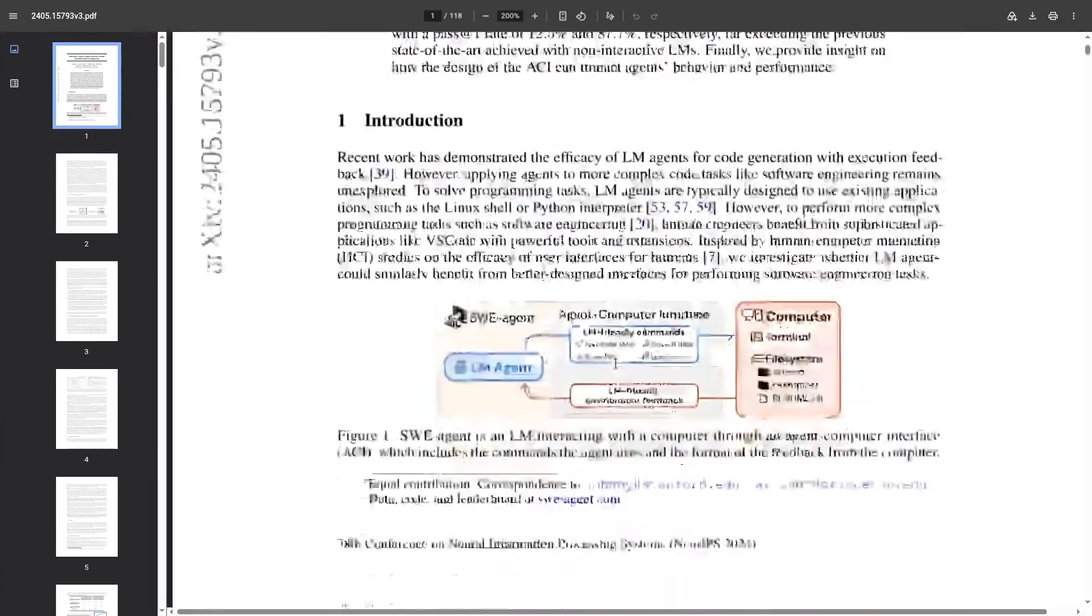
\includegraphics[width=0.92\textwidth]{figures/fig_21_swe_agent_aci_architecture.png}
\caption{2024年 \texttt{SWE-agent} 论文精读：专门为大模型设计的 Agent-Computer Interface（ACI），让智能体能够顺畅地浏览代码、编辑文件并执行测试\vtag}
\end{figure}
\srcnote{00:53:30--00:53:45}

\begin{figure}[H]
\centering
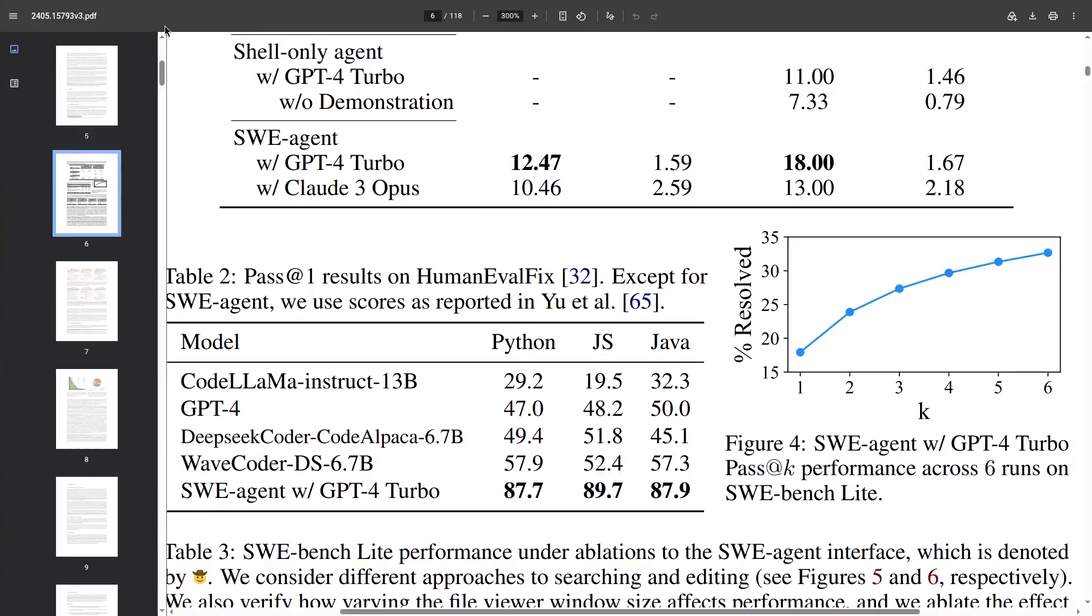
\includegraphics[width=0.92\textwidth]{figures/fig_22_swe_agent_benchmark_results.png}
\caption{\texttt{SWE-agent} 评测结果：对比一次性生成补丁（Zero-shot / 无执行反馈），允许智能体在多轮交互中运行测试并观察报错反馈，使其在 SWE-bench 上的问题解决率实现数量级跃升\vtag}
\end{figure}
\srcnote{00:54:30--00:54:45}

为什么早期让大模型直接根据 GitHub Issue 一次性生成代码补丁（One-shot Patch Generation）的成功率惨不忍睹，而 \texttt{SWE-agent} 却能实现质的飞跃？论文揭示的核心秘诀在于两点：
\begin{enumerate}
    \item \textbf{定制化的人机交互接口（Agent-Computer Interface，ACI）}：人类程序员习惯使用 VS Code 或 Vim 等全屏终端编辑器，但大模型直接在原始 Bash 里操作很容易迷失在几千行的文件输出或语法错误中。\texttt{SWE-agent} 专门为 Agent 设计了一套带行号窗口浏览、带语法静态检查（Lint-gated Edit）的文件编辑与测试执行接口（ACI），大幅降低了模型与计算机交互的摩擦损耗。
    \item \textbf{“写代码 $\to$ 运行测试 $\to$ 观察反馈 $\to$ 再修改”的闭环迭代}：观察图 22 右侧的累积解决率随交互轮次（Turns）增长曲线可以发现，即便是最先进的基底大模型，在第 1 轮直接写对补丁的比例也很有限；绝大多数复杂的真实 Bug，都是模型先写出一个初步实现或复现脚本，**通过调用测试运行器看到真实的报错栈（Traceback）或断言失败信息，再根据这些确定性的客观反馈一步步修正代码，在 10 到 30 轮闭环交互内收敛到正确解的**！
\end{enumerate}

\begin{importantbox}{生成式软件工程核心洞察：测试即 Agent 的环境梯度}
在强化学习与智能体工程中，一段没有测试、不可执行的静态代码是没有反馈信号的“盲写”；而一套快速、精准、可重复的自动化测试套件，本质上就是为 Coding Agent 提供了**无幻觉的外部真实世界反馈（Ground-Truth Feedback）**。你为项目建设的测试与断言越完善，Agent 自己发现错误、自己修好 Bug 的闭环能力就越强！
\end{importantbox}

\subsection{本章小结}

本章剖析了“在我机器上能跑”背后的广义输入空间（跨平台环境、\texttt{package-lock.json} 锁文件、系统时间 \texttt{gettimeofday()}、负载与 CHESS 并发调度交错），结合 Dijkstra 名言与 $1/n!$ 数学概率阐明了测试建立工程信心的原理，并通过 2024年 \texttt{SWE-agent} 论文揭示了执行测试反馈闭环对智能体编程的决定性作用。

% =========================================================================
% SECTION 6
% =========================================================================
\section{经典软件工程测试体系：层次、黑盒/白盒设计与工程化}

\subsection{从局部到整体的四个测试层次与火星气候轨道器事故}

既然测试如此重要，面对一个拥有 100万行代码的庞大软件系统，传统软件工程教科书总结出了哪些系统化的测试方法？蒋老师在幻灯片第 12 至 16 页（图 23 至图 28）中，用一套高屋建瓴的框架带我们快速打通了经典软件工程的测试体系。首先是**按观察边界从小到大划分的四个测试层次**（图 23）：

\begin{figure}[H]
\centering
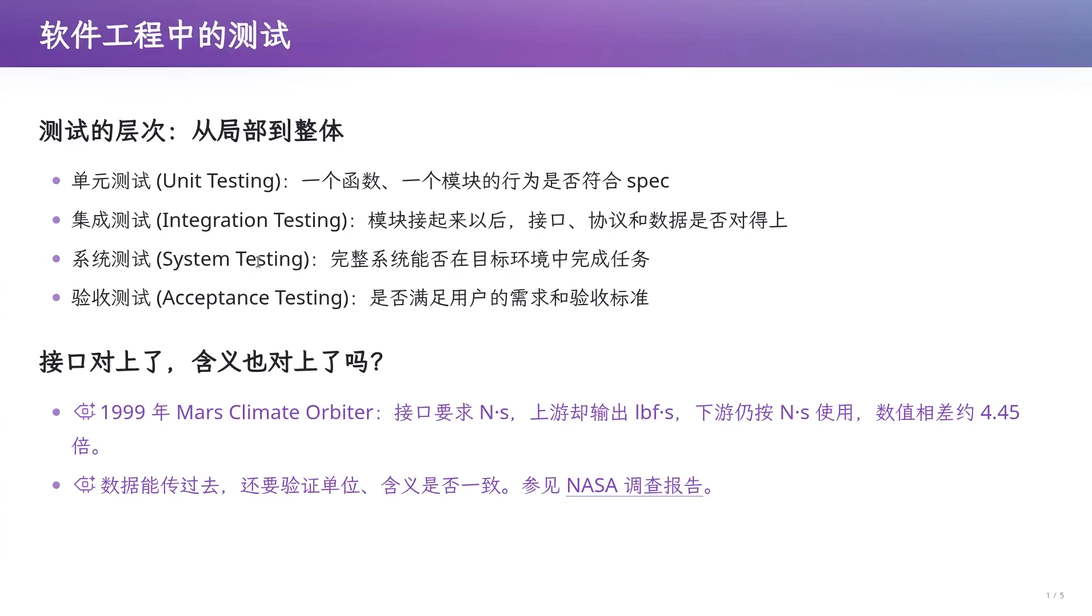
\includegraphics[width=0.92\textwidth]{figures/fig_23_four_testing_levels_mars.png}
\caption{软件工程中的四个测试层次（单元、集成、系统、验收）与 1999 年 NASA 火星气候轨道器因接口单位失配（$\mathrm{lbf\cdot s}$ vs $\mathrm{N\cdot s}$）引发的坠毁事故\vtag}
\end{figure}
\srcnote{00:56:00--00:56:15}

以一个高校教务选课系统为例，四个测试层次各自守卫着不同的质量边界：
\begin{enumerate}
    \item \textbf{单元测试（Unit Testing）——验证单个函数或最小模块是否符合局部规约}：
    把选课系统里的“判断学生是否满足某门课的先修课要求”单独抽出来写成函数 \texttt{check\_prereq(courses, reqs)}。单元测试不连数据库、不启 Web 服务器，直接在内存中传入几组课程列表，毫秒级检验该函数的布尔返回值是否正确。
    \item \textbf{集成测试（Integration Testing）——验证多个模块拼接后接口、协议与数据语义是否对齐}：
    先修课检查函数自己没问题，选课落库模块自己也没问题；但当把它们接在一起时，上游模块传过来的课程编号是形如 \texttt{"CS101"} 的字符串代码，而下游数据库查询接口期待的却是内部自增主键 \texttt{course\_id = 4092}！集成测试专门负责抓出这类“局部都对、拼起来就错”的跨模块接口失配问题。
    \item \textbf{系统测试（System Testing）——验证完整系统在目标运行环境中能否端到端完成任务}：
    将前端页面、后端网关、业务逻辑服务、数据库与缓存完整部署起来，模拟真实浏览器发起从“登录 $\to$ 搜索课程 $\to$ 点击选课 $\to$ 刷新课表”的全链路请求，同时检验高并发抢课下的性能与权限隔离。
    \item \textbf{验收测试（Acceptance Testing）——站在用户与业务方视角验证是否满足真实需求}：
    哪怕代码逻辑完全不崩、性能飞快，但如果教务处的核心业务规约要求“课程人数达到上限后严禁普通选课通道超额选入”，而系统却允许第 $101$ 个学生直接选进容量为 $100$ 的教室，那么它在验收测试阶段就会被一票否决。
\end{enumerate}

在讲解**集成测试（Integration Testing）**时，幻灯片第 12 页底部引用了一个震惊 aerospace 界的真实历史事故——**1999 年 NASA 火星气候轨道器（Mars Climate Orbiter）坠毁事件**：
\begin{itemize}
    \item \textbf{接口类型完全对上了，但物理量的“单位含义”却错位了}：该探测器由洛克希德·马丁公司（Lockheed Martin）负责研制地面推进器冲量计算软件，由 NASA 喷气推进实验室（JPL）负责研制轨道导航软件。两个软件模块之间通过标准数据文件接口传输推进器产生的冲量（Impulse）浮点数，数据类型与通信协议 100\% 匹配，从未发生任何语法报错。
    \item \textbf{英制与公制的致命鸿沟（相差约 $4.45$ 倍）}：NASA 的接口规约文档（SIS）明确规定冲量单位必须采用公制（国际单位制）的**牛顿·秒（$\mathrm{N\cdot s}$）**；然而洛克希德·马丁团队编写的上游软件却按美国工程习惯输出了英制的**磅力·秒（$\mathrm{lbf\cdot s}$）**！由于 $1\,\mathrm{lbf} \approx 4.44822\,\mathrm{N}$，下游导航系统把数值小了 $4.45$ 倍的英制数字当成公制读入，导致长达数月的航行轨迹修正计算持续累积偏差，最终使耗资数亿美元的探测器以过低高度切入火星大气层而彻底焚毁。
\end{itemize}
这一案例深刻说明：**集成测试绝不能只看“接口能不能调通、字段类型是不是 \texttt{float}”，更要验证上下游对数据单位、坐标系、空值语义、错误码约定是否真正达成了一致！**

\subsection{黑盒测试 vs 白盒测试：覆盖率 $100\%$ 就等于代码正确吗？}

确定了测试层次之后，具体到某一个模块，我们究竟该从浩瀚的输入空间里挑选哪些输入来构造测试用例（Test Cases）？软件工程给出了两条互补的路线：**从规约（Spec）出发的黑盒测试**（图 24）与**从代码（Code）出发的白盒测试**（图 25）。

\begin{figure}[H]
\centering
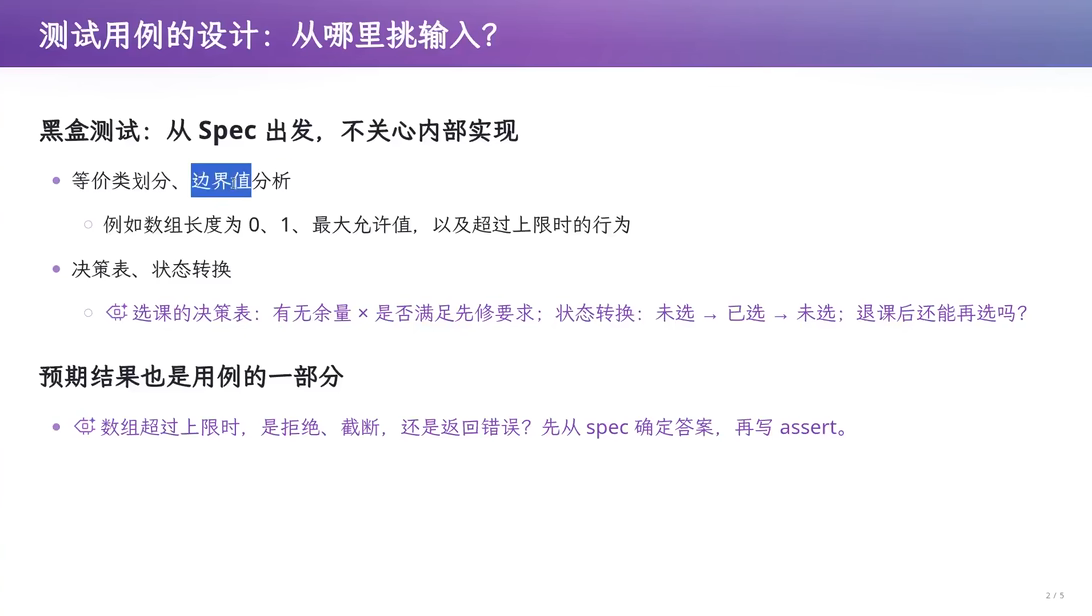
\includegraphics[width=0.92\textwidth]{figures/fig_24_blackbox_testing_design.png}
\caption{黑盒测试用例设计：从规约（Spec）出发，综合运用等价类划分、边界值分析、决策表与状态转换图，且必须将预期结果作为用例的一部分\vtag}
\end{figure}
\srcnote{00:57:45--00:58:00}

\subsubsection{黑盒测试（Black-Box Testing）：不看内部实现，只看规约边界}
在黑盒测试视角下，程序是一个看不见内部源码的黑盒子，我们完全依据规约说明书来挑选最具代表性的输入“子弹”：
\begin{enumerate}
    \item \textbf{等价类划分（Equivalence Partitioning）}：若规约规定课程容量上限为 $100$ 人，那么已选人数为 $35$ 人、$36$ 人、$50$ 人在逻辑上走的是同一个“正常有余量”等价类，无需把 $2 \sim 98$ 逐个测一遍，从中挑选一个代表值（如 $50$）即可；同理，从“负数非法输入”、“正常范围内”、“超过上限”各等价类中分别挑选代表值。
    \item \textbf{边界值分析（Boundary Value Analysis）}：大量手滑 Bug（如把 \texttt{<} 写成 \texttt{<=} 的 Off-by-one Error）都集中在等价类的交界处！因此针对上限 $100$ 的数组或选课容量，必须重点测试 **$0$（空边界）、$1$（最小正数）、$99$（上限减一）、$100$（恰好满额上限）、$101$（刚刚越过上限）**。
    \item \textbf{决策表（Decision Table）}：当业务结果取决于多个布尔条件的组合时（例如选课是否成功同时取决于 $C_1=\text{“课程是否有余量”}$ 与 $C_2=\text{“学生是否满足先修要求”}$），通过 $2 \times 2 = 4$ 行的决策表显式列出 $(\text{是},\text{是})\to\text{成功}$、$(\text{是},\text{否})\to\text{拒选并提示缺先修课}$、$(\text{否},\text{是})\to\text{拒选并提示满员}$、$(\text{否},\text{否})\to\text{拒选}$ 四种组合，防止漏测复合条件。
    \item \textbf{状态转换测试（State Transition Testing）}：许多软件是有状态的。对于选课状态机 $\text{未选} \xrightarrow{\text{选课}} \text{已选} \xrightarrow{\text{退课}} \text{未选}$，除了测试正常正向流转外，还必须测试“在已选状态下重复点击选课”、“在未选状态下直接点击退课”以及“退课之后能否再次重新选上”等状态跃迁路径。
    \item \textbf{预期结果（Test Oracle）是用例不可分割的一部分}：在动手写测试代码之前，必须先从规约中明确“当数组长度超过上限 $100$ 时，系统究竟应该静默截断前 $100$ 个元素、返回错误码 \texttt{-EINVAL}，还是抛出异常？”——没有明确预期结果的测试只是一次盲目的运行。
\end{enumerate}

\newpage
\subsubsection{白盒测试（White-Box Testing）与覆盖率假阳性陷阱}
黑盒测试只看规约，但如果程序员在代码里悄悄写了一个规约里没提的特殊分支（例如某种缓存加速路径或后门条件），黑盒测试可能永远猜不到要去测那个分支。于是我们还需要打开盒子看源码，用**代码覆盖率（Code Coverage）**来度量测试执行过了哪些逻辑（图 25）：

\begin{figure}[H]
\centering
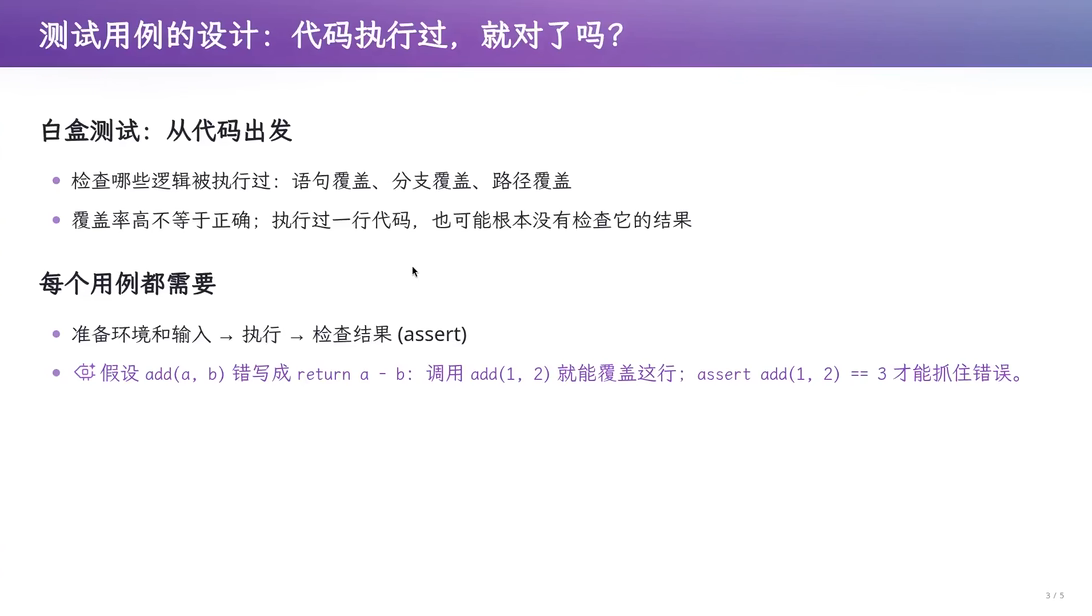
\includegraphics[width=0.92\textwidth]{figures/fig_25_whitebox_coverage_oracle.png}
\caption{白盒测试与覆盖率陷阱：语句覆盖、分支覆盖与路径覆盖的区别，以及为什么 \texttt{add(a, b)} 错写成 \texttt{return a - b} 时仅靠执行覆盖无法发现错误\vtag}
\end{figure}
\srcnote{00:59:15--00:59:30}

\begin{itemize}
    \item \textbf{语句覆盖（Statement / Line Coverage）}：源代码中的每一行可执行语句是否至少被执行过一次？如果某几行代码在所有测试跑完后覆盖率为 $0\%$，说明现有测试集对那片区域是完全失明的。
    \item \textbf{分支覆盖（Branch Coverage）}：每一个 \texttt{if / else}、\texttt{switch} 判断的真假两个方向是否都被走过？注意：对于单行不带 \texttt{else} 的语句 \texttt{if (x > 0) y = 1;}，只需传入 $x = 1$ 即可达到 $100\%$ 语句覆盖，但此时 $x \le 0$ 的假分支根本没测到！分支覆盖要求必须同时测 $x > 0$ 与 $x \le 0$。
    \item \textbf{路径覆盖（Path Coverage）}：要求覆盖从函数入口到出口的所有可能控制流路径组合。若有 $k$ 个独立的顺序 \texttt{if} 语句，路径数就有 $2^k$ 条；一旦包含循环或并发交错，路径数量会瞬间发生组合爆炸，无法穷尽。
\end{itemize}

课堂上，蒋老师特别强调了一个在工业界极其普遍的误区——**把“高覆盖率（甚至达到 100\% 覆盖率）”等同于“高测试质量”**！请看幻灯片第 14 页底部给出的极简反例：

\begin{lstlisting}[language=Python, caption={覆盖率达到 100\% 但完全漏掉 Bug 的反例与正确断言}]
def add(a, b):
    return a - b   # FAULT: programmer wrote '-' instead of '+'

# Bad Test 1: 100% statement/branch/path coverage, ZERO assertions!
def test_add_coverage_only():
    add(1, 2)      # Executes line 2 -> 100% coverage! Test passes!

# Bad Test 2: Coincidental correctness (Fault does not trigger Error)
def test_add_weak_input():
    assert add(1, 0) == 1   # 1 - 0 == 1 + 0 == 1 -> Passes by coincidence!

# Good Test: Arrange -> Act -> Assert with discriminating input + Oracle
def test_add_correct():
    assert add(1, 2) == 3   # 1 - 2 == -1 != 3 -> Immediate AssertionError!
\end{lstlisting}

我们可以将“一个缺陷能否被测试套件捕获”形式化为以下三个充要条件的逻辑合取（又称为 **RIPR 模型：Reachability, Infection, Propagation, Revealability**）：

\begin{equation}
\mathrm{Det}(F, T)
\iff
\exists\, (x, \mathrm{Orc}) \in T:\;
\underbrace{\mathrm{Reach}(x, F)}_{\text{1. 覆盖可达}}
\;\wedge\;
\underbrace{\big(s_{\mathrm{impl}}(x) \neq s_{\mathrm{spec}}(x)\big)}_{\text{2. 触发 Error}}
\;\wedge\;
\underbrace{\big(\neg\,\mathrm{Orc}(x, \mathrm{Impl}(x))\big)}_{\text{3. 断言检出 Failure}}
\end{equation}

上式一针见血地指出了：代码覆盖率达到 100\% 仅仅满足了第 1 项 $\mathrm{Executes}(x, \mathrm{loc}(F))$；如果挑选的输入没有区分度（如 \texttt{add(1, 0)} 导致第 2 项不成立），或者压根没有编写强有力的结果检查断言 $\mathrm{Oracle}$（如只调用 \texttt{add(1, 2)} 而不检查返回值等于 $3$，导致第 3 项不成立），那么就算覆盖率刷到 100\%，测试也只是自欺欺人的数字游戏！每一个合格的测试用例都必须完整包含 **准备环境与输入（Arrange）$\to$ 执行被测代码（Act）$\to$ 用断言检查输出与状态（Assert）** 三步闭环。

\begin{importantbox}{测试神谕（Test Oracle）铁律：没有 Assert 的 100\% 覆盖率只是自欺欺人}
在审查人类或 Coding Agent 编写的单元测试时，绝不能只看测试是否跑通、行覆盖率是否达到 100\%，而必须重点审查其 **\texttt{assert} 语句（Test Oracle）的强度**：
\begin{enumerate}
    \item 是否只断言了“返回值非空（\texttt{assert res is not None}）”或“状态码为 200”，却漏掉了对核心业务计算数值与副作用状态的精确核对？
    \item 输入样本是否避开了恒等退化点（如加法中的 $b=0$、乘法中的 $b=1$），具备真正区分正确实现与错误实现的鉴别力？
\end{enumerate}
\end{importantbox}

\subsection{“测试工程师进酒吧”漫画与日常测试工程化（金字塔、Mock、CI）}

在讲完黑盒与白盒方法后，幻灯片第 15 页展示了一幅软件工程界家喻户晓的幽默漫画——**《A QA engineer walks into a bar》（一个测试工程师走进一家酒吧）**（图 26）：

\begin{figure}[H]
\centering
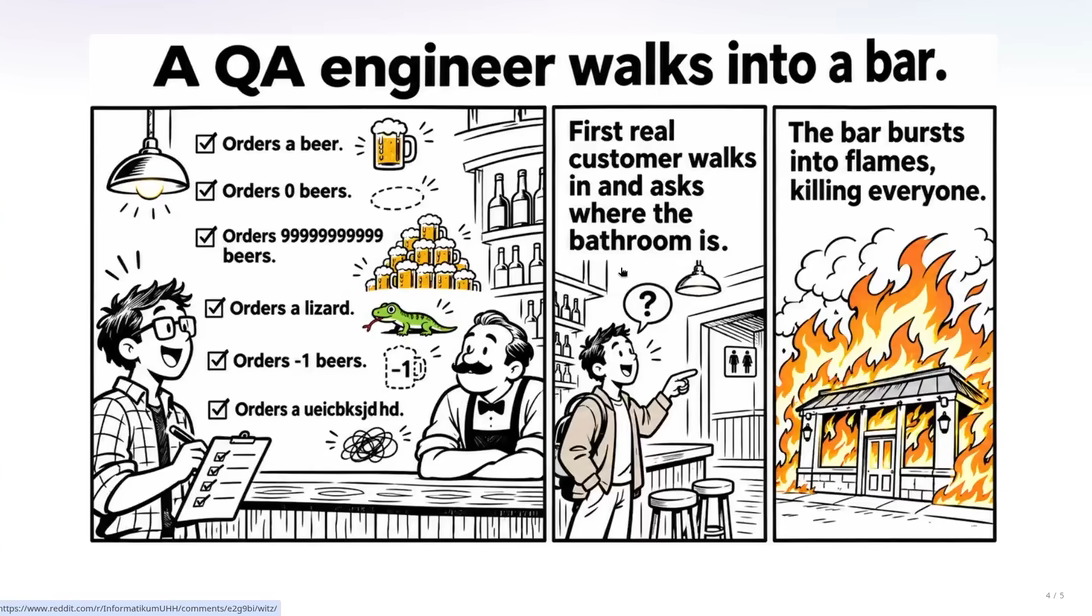
\includegraphics[width=0.92\textwidth]{figures/fig_26_qa_engineer_bar_comic.png}
\caption{《测试工程师进酒吧》漫画：测试工程师用 $0$ 杯、$999999999$ 杯、一只蜥蜴、$-1$ 杯和乱码把点酒接口测了个底朝天，结果第一位真实顾客进门问“厕所在哪”，整个酒吧当场起火爆炸\vtag}
\end{figure}
\srcnote{01:01:00--01:01:15}

漫画的情节令人捧腹却又无比真实：测试工程师走进刚开业的酒吧，极其专业地按边界值分析与非法等价类点了一杯酒、点 $0$ 杯酒、点 $999999999$ 杯酒、点一只蜥蜴、点 $-1$ 杯酒、点一串乱码 \texttt{qwertyuiop}，酒吧系统全部优雅地处理通过；测试工程师心满意足地宣布系统完美上线。结果第一位真实顾客走进酒吧，既没点负数杯也没点蜥蜴，只是问了一句**“请问厕所在哪？”**——整个酒吧瞬间燃起熊熊大火，所有人葬身火海！

这个笑话为什么深刻？因为它讽刺了机械套用教科书测试套路的通病：**如果你只盯着单个接口的参数边界（点多少杯酒）穷追猛打，却对真实用户在完整使用场景下的状态空间与意外交互路径（去上厕所）缺乏系统级理解，再刁钻的参数测试也防不住系统在真实世界里瞬间崩溃。**

接着，幻灯片第 16 页（图 27）与讲义梳理视图（图 28）总结了如何把测试变成可持续的日常工程实践：

\begin{figure}[H]
\centering
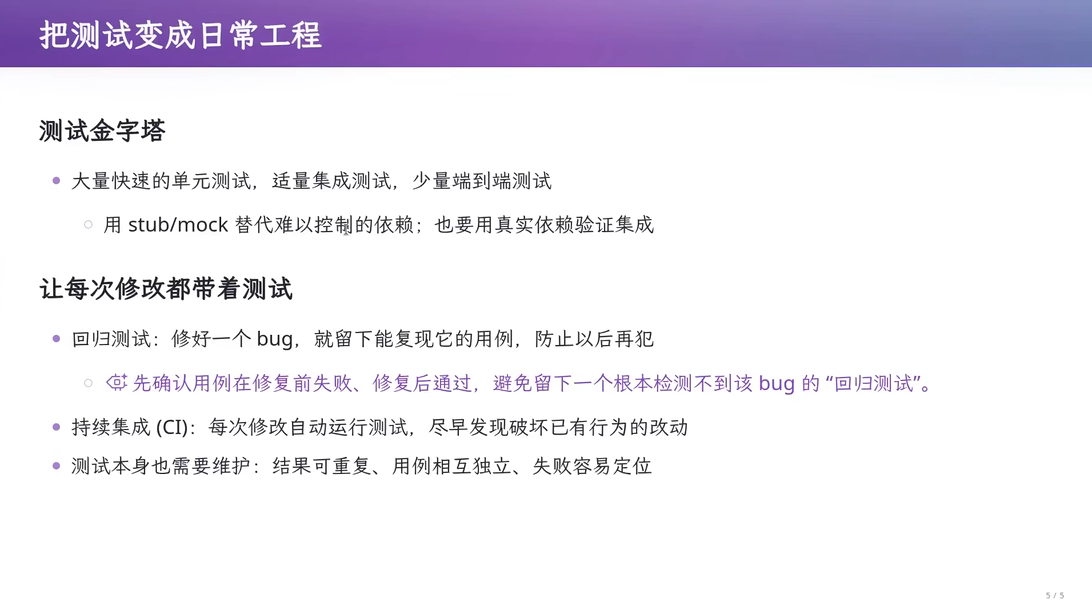
\includegraphics[width=0.92\textwidth]{figures/fig_27_test_pyramid_ci_regression.png}
\caption{把测试变成日常工程：测试金字塔（单元/集成/端到端配比）、Stub/Mock 替身、回归测试（先确认修复前失败）与持续集成（CI）\vtag}
\end{figure}
\srcnote{01:04:15--01:04:30}

\begin{figure}[H]
\centering
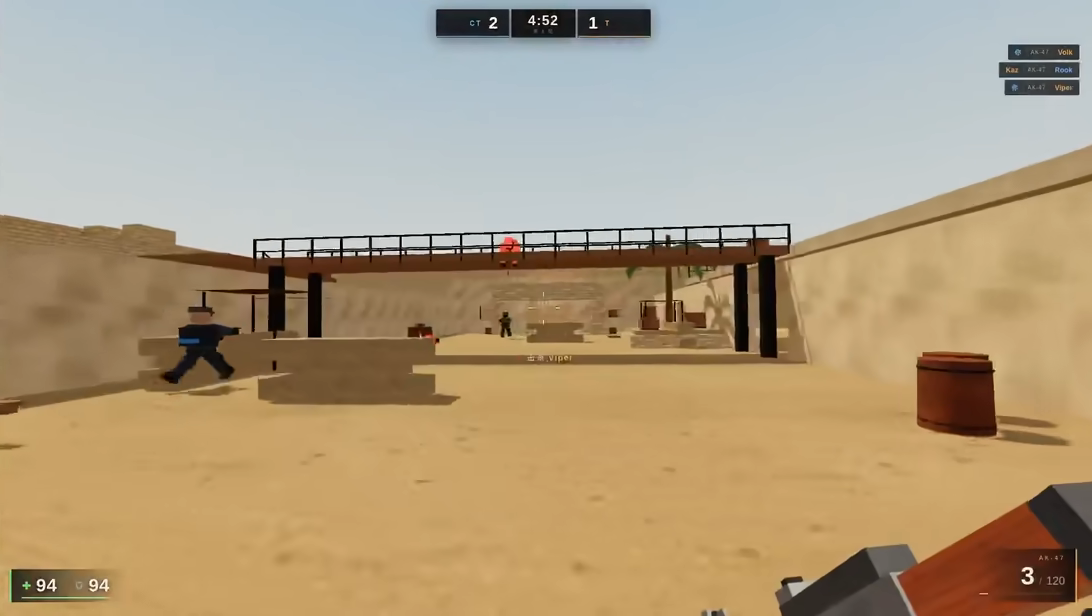
\includegraphics[width=0.92\textwidth]{figures/fig_28_lecture_notes_testing_summary.png}
\caption{课程讲义梳理：传统软件工程测试理论体系与日常工程化实践要点\vtag}
\end{figure}
\srcnote{01:07:30--01:07:45}

\begin{knowledgebox}{日常测试工程化的四大支柱}
\begin{enumerate}
    \item \textbf{测试金字塔（Test Pyramid）——好钢用在刀刃上的子弹经济学}：
    每一个测试用例都是一颗射向规约空间的“子弹”，而不同子弹的造价天差地别。**单元测试**不启外围服务，一秒钟能打几千颗子弹，应当作为金字塔宽阔的底座（数量最多）；**集成测试**需要连接数据库或模块接口，位居金字塔中层（数量适中）；**端到端系统测试（E2E）**需要拉起完整浏览器与后端集群，运行慢、开销大、维护脆弱，应当作为金字塔尖（少量核心主链路）。
    \item \textbf{测试替身（Stub 与 Mock）及其双刃剑效应}：
    当被测模块依赖外部银行支付网关或第三方短信平台时，我们不可能在每次单测时真的去扣银行卡里的钱。此时需引入测试替身：**Stub（桩）**用于向被测代码提供预设的返回结果（如强制模拟“银行返回余额不足”或“网络超时”以测试异常分支）；**Mock（模拟对象）**用于验证被测代码对外部依赖的调用行为（如断言“结账成功时恰好向网关发起 $1$ 次扣款请求，绝未重复扣款”）。但必须警惕：替身毕竟是你自己假想出来的外部世界，仍需配合少量真实依赖集成测试来防止替身与真实接口脱节。
    \item \textbf{回归测试（Regression Testing）的黄金铁律——“先见红（Fail），再见绿（Pass）”}：
    每当在线上或调试中修好一个 Bug，都必须留下一条专门复现该 Bug 的回归测试用例，防止未来有人重构代码时再次犯错。但这里有一条极其重要的工程纪律：**在提交回归测试前，必须先把你的修复代码临时回退（或在修复前运行该测试），亲眼确认这条新写的测试在旧代码上确实会 FAIL（变红），加上修复代码后才会 PASS（变绿）**！否则你很可能由于配错了测试条件，留下了一条不管 Bug 存不存在都永远 PASS 的“假回归测试”。
    \item \textbf{持续集成（Continuous Integration，CI）与零容忍 Flaky Tests}：
    每次 \texttt{git push} 或发起 Pull Request 时，由 CI 服务器在干净、受控的标准环境里自动全量跑一遍测试。要让 CI 真正发挥防线作用，测试本身必须满足**结果可重复（无随机抽风的 Flaky Tests）、用例间相互独立（不依赖固定执行顺序或残留全局状态）、失败时报错信息清晰易定位**。一旦团队对“有时候红、重跑一次又绿”的抽风测试习以为常，整个 CI 门禁的工程信用就会彻底破产。
\end{enumerate}
\end{knowledgebox}

\subsection{本章小结}

本章系统梳理了经典软件工程的测试矩阵：四个测试层次（及 1999 年火星气候轨道器单位失配教训）、黑盒四大设计法（等价类、边界值、决策表、状态转换）、白盒三大覆盖率（及 \texttt{add(a,b) = a - b} 的 100\% 覆盖假阳性反例）、“测试工程师进酒吧”的场景启示，以及测试金字塔、Stub/Mock、回归测试与 CI 工程化规范。

% =========================================================================
% SECTION 7
% =========================================================================
\section{真实系统的长程任务挑战：从许愿 CS:GO 到“架构决定质量”}

\subsection{许愿一个 CS:GO（\texttt{CS:THREE}）：202 次提交、4,021 行代码与 413 报错}

讲完了教科书上的经典测试理论，蒋老师话锋一转，把目光投向了令全场同学精神振奋的真实世界问题（图 29）：**在今天这个“一天到晚都在向 AI 许愿”的时代，像刚才讲的那些等价类划分、边界值分析，在真实的复杂软件系统里究竟够不够用？**

\begin{figure}[H]
\centering
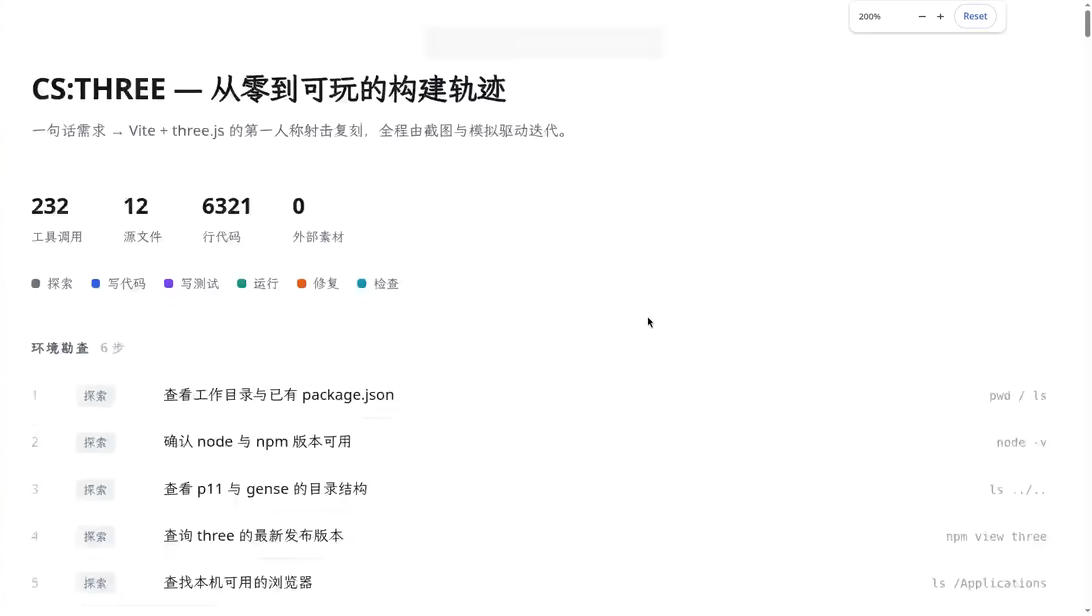
\includegraphics[width=0.92\textwidth]{figures/fig_29_real_world_vibe_coding_era.png}
\caption{真实软件系统的测试挑战：当许愿编程（Vibe Coding）时代来临，我们该如何保障复杂长程任务的质量？\vtag}
\end{figure}
\srcnote{01:08:00--01:08:15}

不管是前两天给家里小朋友在 ESP32 小硬件上许愿做一个仿 Apple Watch 的小界面（内置节拍器、To-Do List 与 AI 聊天工具），还是昨天刚在自己 Mac 上用 \texttt{DeepSeek Harness} 许愿生成的一个大型项目——蒋老师在课堂上直接打开浏览器，现场演示了他向 Agent 许愿开发的一款纯前端 3D 战术射击游戏：**《CS:THREE —— 从零到可玩的战术射击》（网页版 CS:GO）**（图 30、图 31、图 32）！

\begin{figure}[H]
\centering
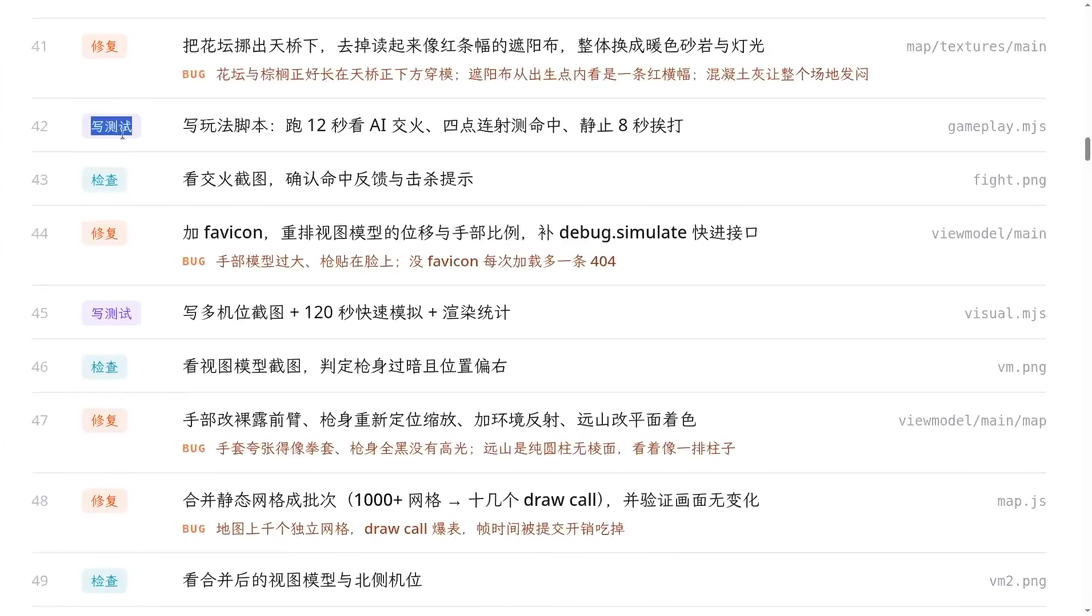
\includegraphics[width=0.92\textwidth]{figures/fig_30_csthree_live_demo_map.png}
\caption{\texttt{CS:THREE} 战术射击游戏实机演示（一）：纯浏览器渲染的 3D 沙城风格地图、掩体箱子与 AI 机器人（BOT）自动寻路交火\vtag}
\end{figure}
\srcnote{01:08:45--01:09:00}

\begin{figure}[H]
\centering
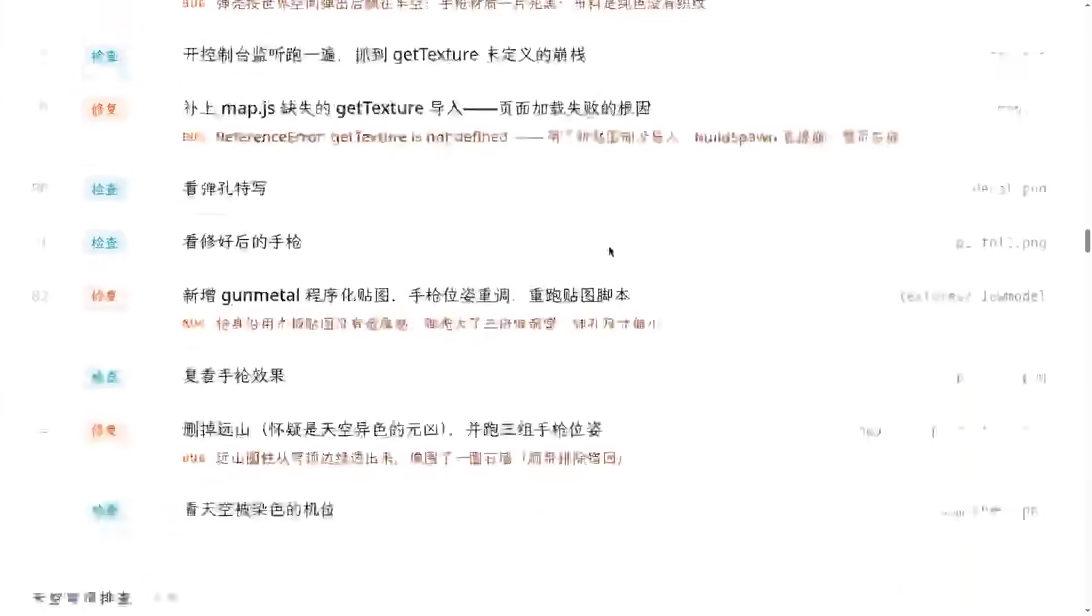
\includegraphics[width=0.92\textwidth]{figures/fig_31_csthree_project_metrics.png}
\caption{\texttt{CS:THREE} 项目演化统计面板：由智能体自主完成 \textbf{202 次 Git 提交、12 个里程碑（Milestones）、4,021 行代码、0 次人工手动编辑}，并附带完整演进时间线\vtag}
\end{figure}
\srcnote{01:09:30--01:09:45}

\begin{figure}[H]
\centering
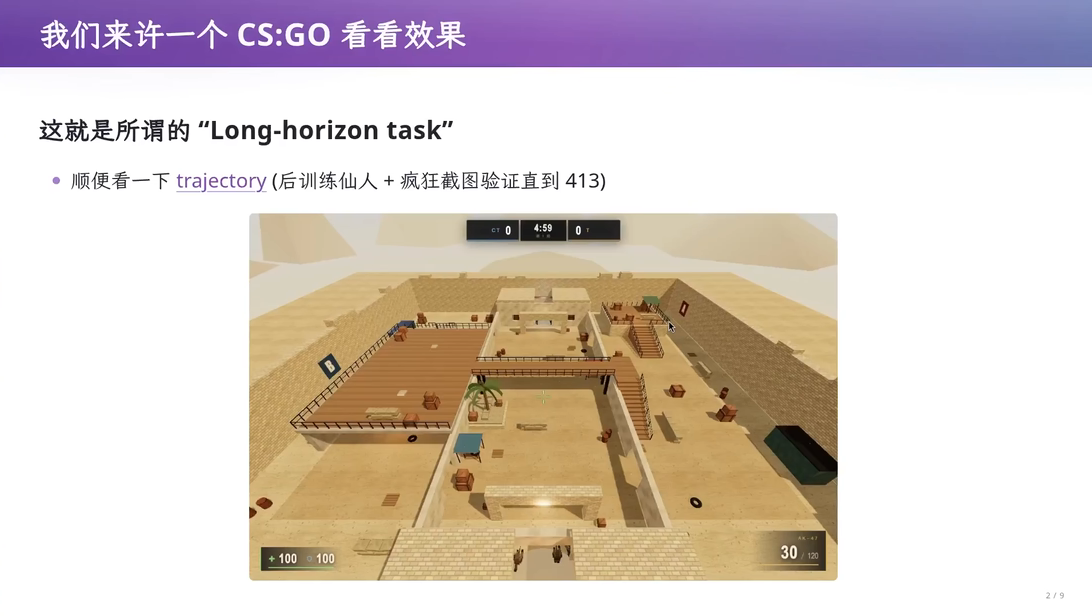
\includegraphics[width=0.92\textwidth]{figures/fig_32_csthree_fps_gameplay.png}
\caption{\texttt{CS:THREE} 战术射击游戏实机演示（二）：第一人称视角持枪建模、动态准星、生命值/护甲/弹药 HUD 与音效反馈\vtag}
\end{figure}
\srcnote{01:11:45--01:12:00}

看看图 31 的统计面板：这个像模像样的 3D 第一人称射击游戏，总共经历了 **202 次提交（Commits）、12 个演进里程碑（Milestones）、4,021 行代码，且人类手动修改行数为 0**！这就是当前大模型领域最热门的所谓 **长程任务（Long-horizon Task）**（图 33）。

那么，Agent 在连续干活好几个小时、写下这 4,021 行代码的过程中，究竟是怎么做测试与质量验证的呢？蒋老师强烈建议所有同学养成一个习惯：**每当 Agent 干完一件大事后，一定要打开它的执行轨迹（Trajectory）复盘它到底干了什么！** 于是我们在课堂上看到了极其戏剧性的一幕（图 33、图 34）：

\begin{figure}[H]
\centering
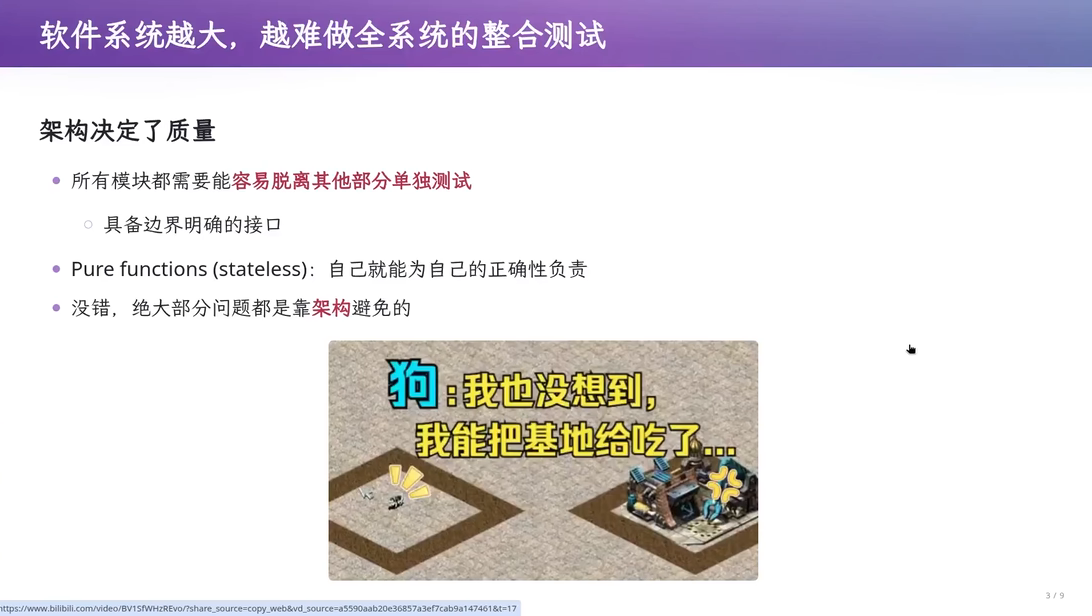
\includegraphics[width=0.92\textwidth]{figures/fig_33_long_horizon_task_slide.png}
\caption{我们来许一个 CS:GO 看看效果：长程任务（Long-horizon Task）中，“后训练仙人”模型通过反复截图验证推进项目，直到触发 HTTP 413 报错\vtag}
\end{figure}
\srcnote{01:13:30--01:13:45}

\begin{figure}[H]
\centering
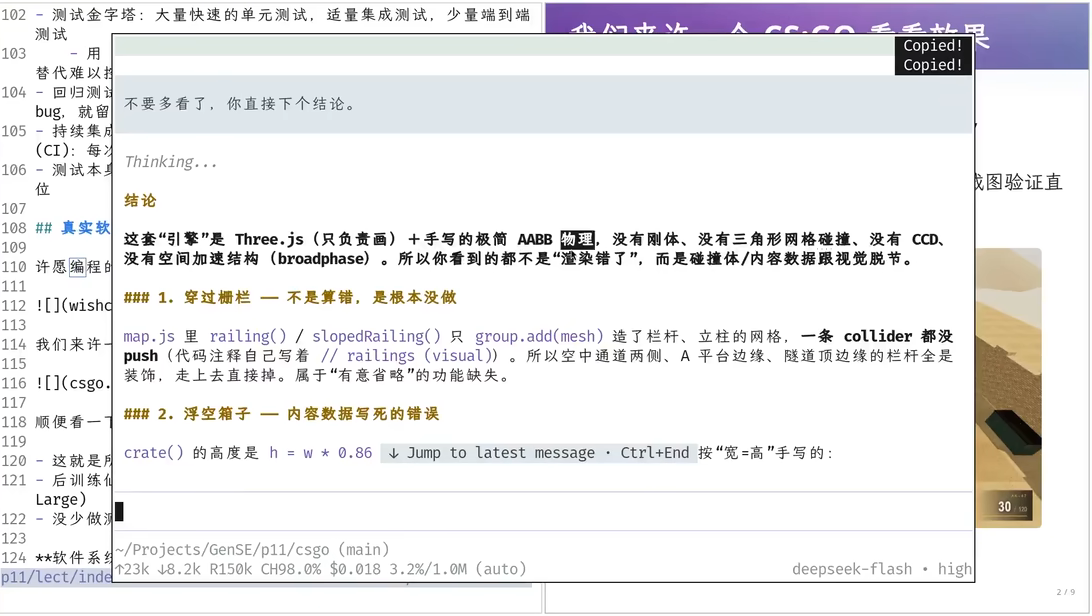
\includegraphics[width=0.92\textwidth]{figures/fig_34_agent_trajectory_http_413.png}
\caption{Agent 执行轨迹（Trajectory）深度复盘：智能体尽职尽责地编写自动玩法脚本、跑 12秒看 AI 交火并截取多机位图片送入上下文，最终因图片 Base64 撑爆请求体而触发 \texttt{413 Payload Too Large}\vtag}
\end{figure}
\srcnote{01:16:00--01:16:15}

\begin{warningbox}{Trajectory 复盘启示录：为什么“后训练仙人”疯狂截图直到 413 依然不够？}
打开 \texttt{CS:THREE} 的智能体执行轨迹（图 34），我们看到现在的“后训练仙人”模型真的极其敬业：
\begin{enumerate}
    \item \textbf{Agent 自发构建了端到端视觉验证闭环}：它不仅写了代码，还主动写了一个自动化玩法脚本，每次修改后自动拉起无头浏览器（Headless Browser），控制角色在地图里跑动、开枪、甚至专门**跑 12秒看 AI 交火**，然后从第一人称、俯视、侧视等多个机位截取 \texttt{screenshot.png} 画面传回给多模态大模型自己看！
    \item \textbf{滑稽的结局——触发 HTTP \texttt{413 Payload Too Large}}：由于它太爱截图了，每轮迭代都把好几张高清游戏截图塞进多轮对话历史（Context）里，跑着跑着上下文体积超过了 API 网关的请求体上限，直接撞上了 \textbf{\texttt{HTTP 413 Payload Too Large}} 错误而中断！
    \item \textbf{更深层的工程瓶颈——端到端截图验证既昂贵又粗糙}：
    哪怕没有遇到 413 报错，靠“启动浏览器渲染 3D 画面 $\to$ 跑 12秒交火 $\to$ 截图肉眼看画面”也是一种极度低效的测试方式！一张截图只能告诉你“箱子贴图渲染出来了、枪口有火光”，却几乎无法精准验证：**“AK-47 打中穿防弹衣的敌人胸部到底扣了多少血？弹匣从 30 发打到 0 发时换弹冷却是不是精确的 2.5 秒？移动跳跃时的散射弹道公式写对了没有？回合倒计时归零瞬间安包判定是否有竞态条件？”**
\end{enumerate}
\end{warningbox}

\subsection{全讲核心命题：软件系统越大，越难整合测试——架构决定了质量！}

为什么 Agent 在测试 \texttt{CS:THREE} 时只能笨拙地去截屏？因为如果你不给 Agent 任何架构约束，它默认写出来的游戏往往是把 **Three.js 3D 渲染、键盘鼠标 DOM 事件监听、物理碰撞检测、武器伤害结算、BOT 决策状态机** 全部揉成一团塞在同一个巨大的循环里！当所有逻辑都和浏览器 WebGL 渲染器死死绑在一起时，除了真的打开浏览器截屏，你根本没有任何办法去单独测试里面的游戏规则！

为此，蒋老师结合模块化游戏实体示意（图 35）与幻灯片第 19 页（图 36），提出了整堂课最核心的工程论断——**“软件系统越大，越难做全系统的整合测试；架构决定了质量（Architecture Determines Quality）！”**

\begin{figure}[H]
\centering
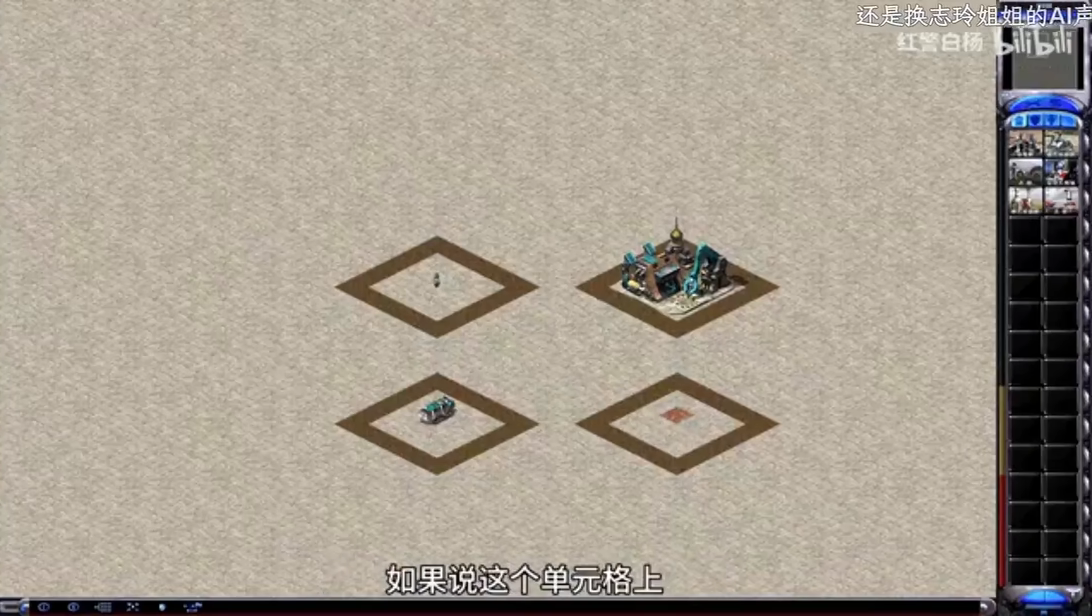
\includegraphics[width=0.92\textwidth]{figures/fig_35_modular_game_entities.png}
\caption{复杂游戏系统的模块化拆解示意：将地图区块、建筑资产、单位状态与渲染表现解耦为边界清晰的独立组件\vtag}
\end{figure}
\srcnote{01:17:15--01:17:30}

\begin{figure}[H]
\centering
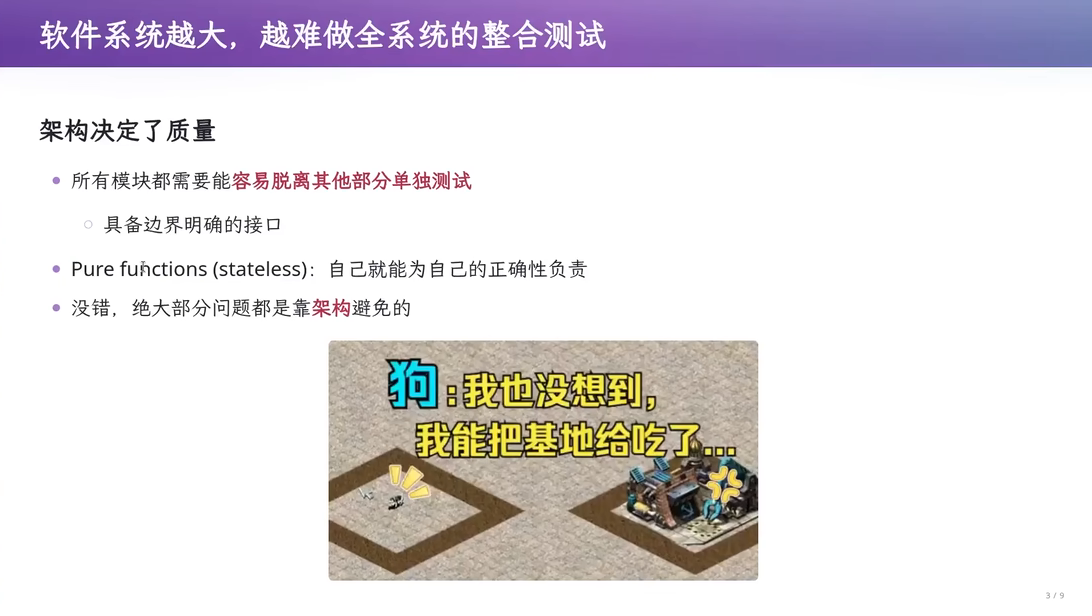
\includegraphics[width=0.92\textwidth]{figures/fig_36_architecture_determines_quality.png}
\caption{架构决定了质量：所有模块都必须能够容易地脱离其他部分单独测试、具备边界明确的接口，并尽可能提取为无状态纯函数（Pure Functions）\vtag}
\end{figure}
\srcnote{01:20:15--01:20:30}

什么样的架构才是“自带高质量基因、极易被人类与 Agent 测试”的好架构？图 36 给出了三条黄金准则：
\begin{enumerate}
    \item \textbf{所有模块都必须能够容易地脱离其他部分单独测试（Isolated Testability）}：正如课堂所举的例子，无论是游戏里的物理引擎、人物移动模块，还是与 Docker 容器通信的接口，都不应该要求“必须先把整个 3D 渲染管线、声卡驱动和网络大厅全部拉起来才能跑测试”。
    \item \textbf{具备边界明确的接口（Well-Defined Interfaces）}：模块与模块之间只通过结构化的数据向量或事件总线（Event Bus）交互，契约边界一清二楚。
    \item \textbf{核心逻辑纯函数化（Pure Functions / Stateless Core）——“自己就能为自己的正确性负责”}：
    如果一个函数是**无状态的纯函数（Pure Function）**——即它的输出 100\% 仅由显式传入的参数决定，不偷偷读取全局时钟、不偷偷调用全局随机数、不直接操作 DOM 或数据库——那么测试它就变得像测试数学函数 $\sin(x)$ 一样简单、飞快且绝对可重复！
\end{enumerate}

\subsection{灵光一闪：可测试性架构的四大工业级范式（游戏状态机、时钟注入、Stripe 幂等键、FoundationDB）}

为了让“通过架构设计消灭测试难题”这一思想落地，幻灯片第 20 页（图 37）浓缩了四个令人拍案叫绝的工业级“灵光一闪”范式：

\begin{figure}[H]
\centering
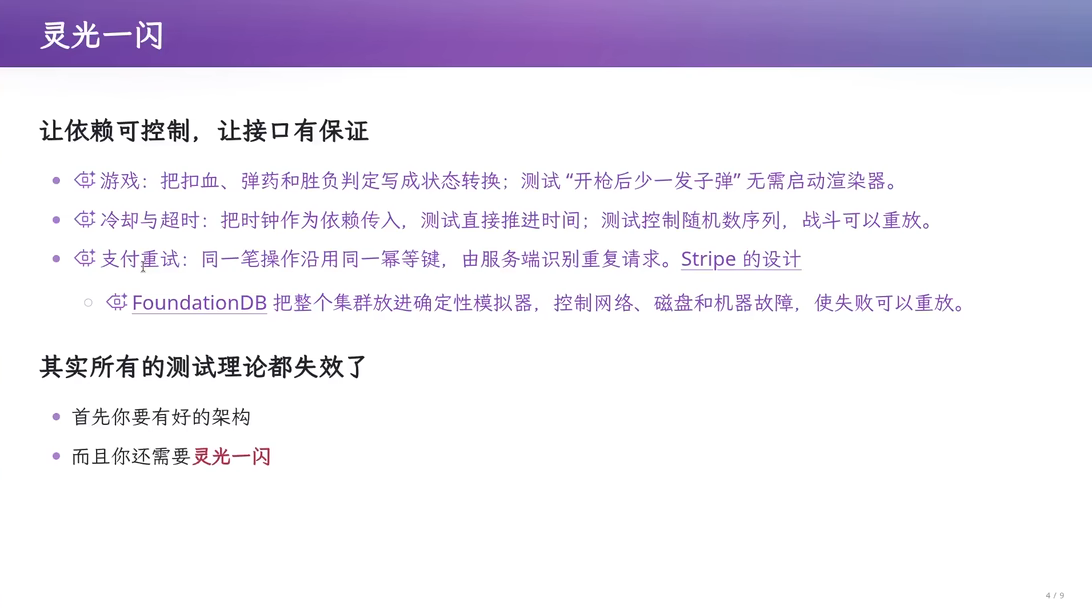
\includegraphics[width=0.92\textwidth]{figures/fig_37_controllable_dependencies_idioms.png}
\caption{可测试性架构的“灵光一闪”：让依赖可控制、让接口有保证——游戏纯状态机、时钟与随机数显式注入、Stripe 支付幂等键以及 FoundationDB 的确定性集群模拟\vtag}
\end{figure}
\srcnote{01:24:15--01:24:30}

我们可以把这四个范式统一抽象为**确定性可重放状态转换方程（Deterministic Replayable State Machine）**：

\begin{equation}
\langle S_{t+1},\; E_{t+1} \rangle
= \mathrm{step}\big(S_t,\; a_t,\; \Delta t_{\mathrm{injected}},\; \xi_t^{\mathrm{seeded}}\big)
\end{equation}

上式中各符号的工程设计意义对应图 37 的四大案例：
\begin{enumerate}
    \item \textbf{游戏逻辑与渲染彻底分离（Game Logic as Pure State Transition）}：
    把 CS:GO 的当前战局（所有玩家的坐标、朝向、生命值 $\mathrm{HP}$、弹匣余量 $\mathrm{ammo}$、回合剩余时间）封装为一个纯数据结构体 $S_t$，把玩家本帧的操作（如 \texttt{Action::Fire} 开火或 \texttt{Action::Reload} 换弹）记为 $a_t$。核心引擎就是一个纯函数 $\mathrm{step}(S_t, a_t) \to \langle S_{t+1}, E_{t+1} \rangle$（其中 $E_{t+1}$ 是发给渲染器与声卡的展示事件，如播放枪声）。如此一来，\textbf{我们要测试“开一枪后弹匣少一发子弹、命中头部扣除对应生命值”，根本不需要启动 Three.js 渲染器、不需要截屏，只需在单元测试里构造一个 JSON 初态 $S_0$，调用一次 $\mathrm{step}(S_0, \mathtt{Fire})$，在 0.1 毫秒内直接断言 $\mathtt{S\_1.ammo == S\_0.ammo - 1}$ 即可！}
    \item \textbf{技能冷却、超时与暴击重放——把时钟 $\Delta t_{\mathrm{injected}}$ 和随机数流 $\xi_t^{\mathrm{seeded}}$ 作为依赖显式传入}：
    如果代码里直接调用操作系统的 \texttt{sleep(30)} 或 \texttt{gettimeofday()} 来判断“30 秒技能冷却是否结束”，那么测试一次冷却就得干等 30 秒，且受机器负载抖动影响极易变成 Flaky Test；如果直接调用系统真随机数算暴击，一旦战斗出现 Bug 就再也无法复现。**可测试性架构的做法是：严禁核心逻辑直接调用系统时钟与全局随机源，而是将虚拟时钟增量 $\Delta t_{\mathrm{injected}}$ 与固定种子伪随机数生成器（Seeded PRNG）$\xi_t^{\mathrm{seeded}}$ 作为参数传入！** 测试时只需一行代码把虚拟时钟拨快 $30.0\,\mathrm{s}$，就能瞬间测完所有超时与冷却边界；只要保存初始状态 $S_0$、随机种子 $\mathrm{seed}$ 和玩家操作序列 $\{a_t\}$，整场数十分钟的激烈战斗就能在任何机器上一模一样地 100\% 确定性重放！
    \item \textbf{支付重试与接口契约——Stripe 的幂等键（Idempotency Key）设计}：
    在分布式支付系统中，客户端向服务端发起扣款请求时如果遇到网络超时，客户端根本无法得知“刚才那笔请求到底是在去往服务端的路上丢了（尚未扣款），还是服务端已经扣款成功但返回响应在回来的路上丢了”。如果贸然重试，就会造成可怕的重复扣款！在线支付巨头 **Stripe** 是如何用架构解决这个测试与容错难题的？它要求客户端为同一笔业务操作生成一个全局唯一的**幂等键（\texttt{Idempotency-Key}）**，并在网络重试时沿用同一个幂等键：
    \begin{equation}
    \forall\, k \in \mathcal{K}_{\mathrm{idemp}},\quad
    \mathrm{Pay}(k, \mathrm{req}) \circ \mathrm{Pay}(k, \mathrm{req}) = \mathrm{Pay}(k, \mathrm{req})
    \end{equation}
    服务端一旦发现收到的 \texttt{Idempotency-Key} $k$ 已经处理过，就绝不重复执行扣款逻辑，而是直接原样返回上一次记录的处理结果。通过将接口设计为幂等的（见上式），网络抖动与重试问题在架构层面就被优雅地消解了。
    \item \textbf{分布式集群的终极检验——FoundationDB 的确定性仿真（Deterministic Simulation Testing）}：
    如果我们要开发一个运行在 100台服务器集群上的工业级分布式数据库，面对网络分区、交换机丢包、磁盘静默损坏、机器突然断电重启等海量故障组合，怎么可能真去买 100台服务器天天拔网线、拔电源来测试？
    分布式数据库先驱 **FoundationDB**（后被 Apple 收购并成为 CloudKit 底座）做出了一个惊世骇俗的架构决定：**在写第一行数据库业务代码之前，先用带确定性伪随机调度的单线程事件循环模拟器（Flow 语言与仿真框架），把整个 100台服务器的集群、网络延迟、磁盘 I/O 与机器故障全部装进一个单进程虚拟世界里！** 在这个仿真器里，主时钟、网络丢包和磁盘损坏全部由一个随机数种子（Seed）控制，一台普通机器一晚上就能模拟真实世界几万小时的极端故障轰炸；一旦某个种子在跑了十亿步后触发了数据不一致，工程师只需拿着这一个 64 位整数 Seed，就能在自己的笔记本电脑上分毫不差地单步调试整个分布式集群的崩溃瞬间！
\end{enumerate}

正如幻灯片第 20 页底部那句掷地有声的总结：**“面对复杂的真实系统，其实教科书上所有的常规测试理论都失效了——首先你要有好的架构，而且你还需要一点灵光一闪！”**

\subsection{本章小结}

本章通过现场复盘 4,021 行代码的 \texttt{CS:THREE} 长程任务及其 HTTP 413 截图报错轨迹，深刻阐明了“架构决定软件质量”的第一性原理，并拆解了纯函数状态机、时钟/随机数依赖注入、Stripe 幂等键与 FoundationDB 100台服务器级确定性仿真四大工业范式。

% =========================================================================
% SECTION 8
% =========================================================================
\section{灵光一闪（一）：差分测试（Differential Testing）——从 NEMU 到香山}

\subsection{为什么复杂系统最缺的是 Test Oracle？——2013 年 NEMU 与《仙剑奇侠传》跑飞}

在上式中我们看到，任何测试要想抓住 Bug，都离不开一个能够判断“当前输出和状态到底对不对”的裁判——即 **测试神谕（Test Oracle）**。对于 \texttt{add(1, 2) == 3} 这样的小函数，人类一眼就能写出 Oracle；但如果我们要测试的是一个完整的 C 语言编译器（GCC / LLVM）、一个数据库执行引擎（SQLite），或者一个完整的计算机系统模拟器（如南京大学计算机系从 2013年左右开始创立并延续至今的《计算机系统基础》PA 大作业教学模拟器 **NEMU**），Test Oracle 从哪里来？

\begin{figure}[H]
\centering
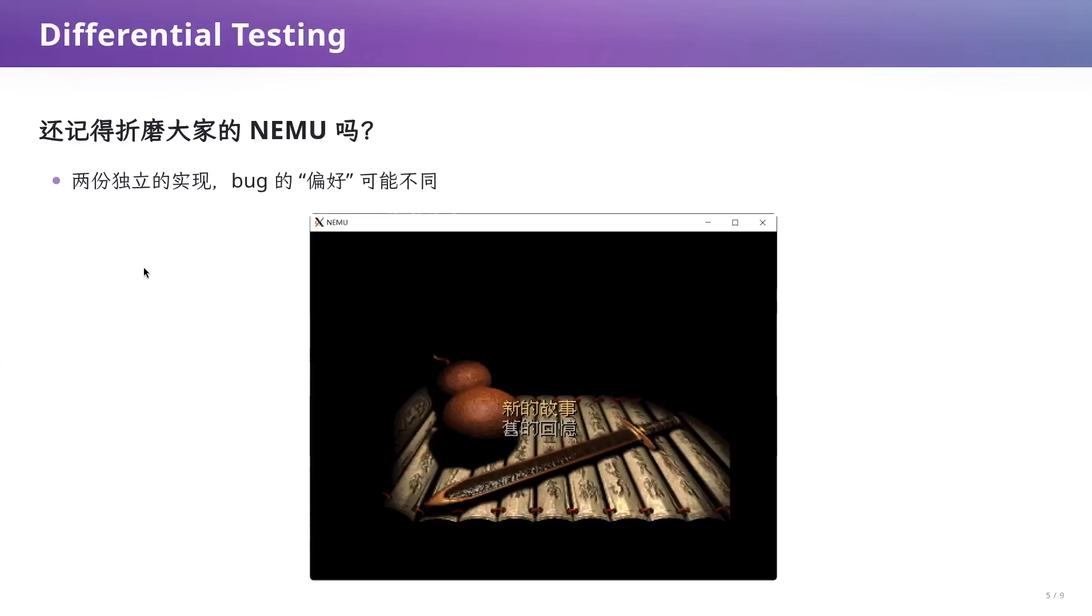
\includegraphics[width=0.92\textwidth]{figures/fig_38_differential_testing_nemu.png}
\caption{差分测试（Differential Testing）的引出：还记得折磨大家的 NEMU 吗？两份独立编写的实现，手滑犯错的“偏好”往往分布在不同的地方\vtag}
\end{figure}
\srcnote{01:26:45--01:27:00}

蒋老师在课堂上深情回顾了 2013年创立 NEMU 时的亲身经历（图 38、图 39）：当时要求本科生从零用 C 语言实现一个能跑起操作系统的 x86 / RISC-V / MIPS 全系统指令集模拟器（NEMU），最终的终极验收目标是把经典游戏《仙剑奇侠传》完整跑起来。然而在没有自动化工具的年代，调试 NEMU 是一场彻头彻尾的噩梦：

\begin{figure}[H]
\centering
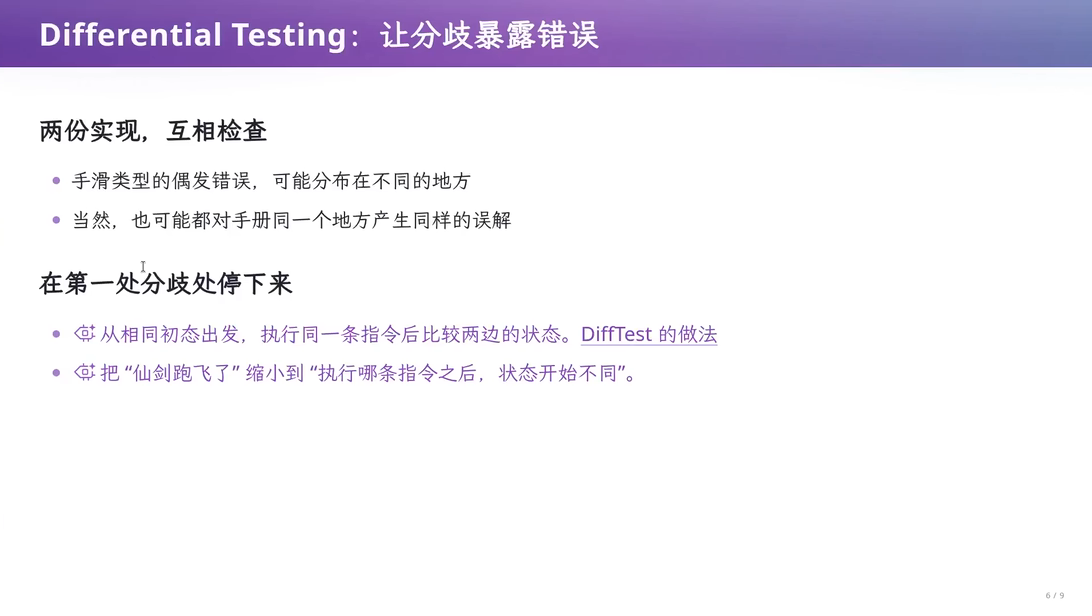
\includegraphics[width=0.92\textwidth]{figures/fig_39_difftest_first_divergence.png}
\caption{DiffTest 的核心机制：让两份实现从相同初态出发，每执行完一条指令就比对一次全套体系结构状态，并在**第一处分歧处当场停下**，将“《仙剑》跑飞了”精准定位到出错的那一条指令\vtag}
\end{figure}
\srcnote{01:29:30--01:29:45}

想象一下：你在实现某一条不常用的位运算指令或条件跳转标志位（\texttt{EFLAGS}）时手滑写反了一个符号（\texttt{Fault}）。当你启动《仙剑奇侠传》时，前五千万条指令一切正常；到了第 $50,000,001$ 条指令执行到那个手滑的指令时，某个通用寄存器或标志位算错了 $1$ 个比特（此时内部已发生 \texttt{Error}，但画面没有任何异常）；接着程序带着这个错了 $1$ 比特的寄存器又继续往前跑了两千万条指令，导致指针偏移算错、跳进了非法内存区，最终在第 $70,000,000$ 条指令处屏幕花屏崩溃（\texttt{Failure}，“仙剑跑飞了”）！如果你在崩溃的第 $70,000,000$ 条指令处挂上 GDB 调试器，看到满目疮痍的寄存器与栈内存，你根本不可能倒推回两千万条指令之前去找到最初那个手滑的指令！

怎么把从 \texttt{Error} 到 \texttt{Failure} 之间长达两千万条指令的潜伏期压缩为零？当时的灵光一闪就是——**差分测试（Differential Testing，简称 DiffTest）**！

\subsection{DiffTest 的数学原理与香山（XiangShan）处理器 4 亿周期实战案例}

虽然我们很难凭空写出一个判断“第 $50,000,001$ 条指令执行后 32 个寄存器应该等于多少”的形式化公式，但世界上已经存在经过长期工业检验的成熟模拟器（如 **QEMU**、RISC-V 官方参考模型 **Spike**，或者已经调通的标准版 **NEMU**）！两份由不同团队独立编写的实现，就算都有手滑 Bug，它们在同一个比特上犯下完全相同手滑错误的概率微乎其微（除非双方都对指令集手册的同一句模糊描述产生了完全相同的误解）。

于是，**DiffTest** 构建了如下逐指令锁步协同验证机制（Lockstep Co-Simulation）：设待测系统（Design Under Test，简称 $\mathrm{DUT}$）的状态转移函数为 $\delta_{\mathrm{DUT}}$，参考黄金模型（Reference Model，简称 $\mathrm{REF}$）的状态转移函数为 $\delta_{\mathrm{REF}}$，体系结构可见状态投影（通用寄存器组 $\mathrm{GPR}$、程序计数器 $\mathrm{PC}$、控制与状态寄存器 $\mathrm{CSR}$）为 $\Pi_{\mathrm{arch}}(S)$。我们令两者从完全相同的复位初态 $S_0^{\mathrm{DUT}} = S_0^{\mathrm{REF}} = S_0$ 出发，每执行完单条指令 $k = 1, 2, \dots$，立即执行状态等价性断言：

\begin{equation}
\text{DiffTest Oracle at step } k:\quad
\mathtt{assert}\Big(\Pi_{\mathrm{arch}}\big(\delta_{\mathrm{DUT}}(S_{k-1}^{\mathrm{DUT}})\big) \;==\; \Pi_{\mathrm{arch}}\big(\delta_{\mathrm{REF}}(S_{k-1}^{\mathrm{REF}})\big)\Big)
\end{equation}

一旦在第 $k^*$ 条指令执行完毕的瞬间发现：
\begin{equation}
k^* = \min\Big\{\, k \ge 1 \;\Big|\; \Pi_{\mathrm{arch}}(S_k^{\mathrm{DUT}}) \neq \Pi_{\mathrm{arch}}(S_k^{\mathrm{REF}}) \,\Big\}
\end{equation}
DiffTest 框架当场拉响警报并停机打印出第 $k^*$ 条指令的机器码、指令名以及两边不一致的寄存器值！通过上述方程，原本潜伏两千万条指令才导致“仙剑跑飞”的诡异 Bug，在它刚刚把寄存器算错 $1$ 个比特的那一条指令（$k^*$）处就被当场抓获——**直接把 $\mathtt{Error \to Failure}$ 的传播距离压缩到了 1 条指令（零延迟）！**

更令人自豪的是，这套诞生于南京大学本科教学课堂的 NEMU DiffTest 思想，后来直接走出了教室，成为中国开源高性能 RISC-V 处理器旗舰项目——中科院计算所与鹏城实验室等联合研发的**“香山”（XiangShan）开源乱序执行处理器**——最核心的敏捷验证基础设施（图 40）！

\begin{figure}[H]
\centering
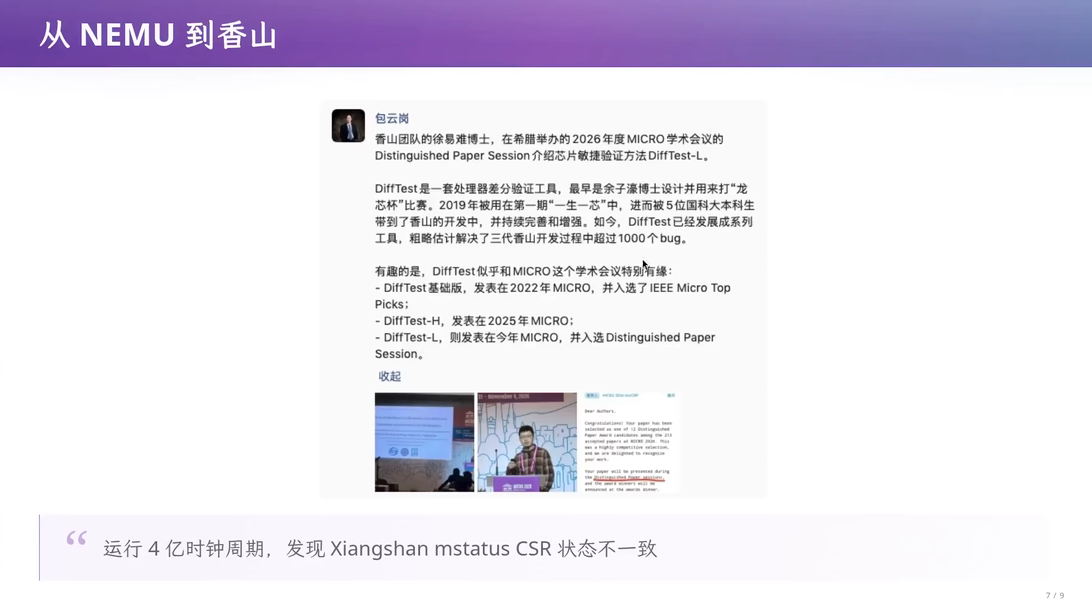
\includegraphics[width=0.92\textwidth]{figures/fig_40_xiangshan_difftest_mstatus.png}
\caption{从 NEMU 教学模拟器到“香山”（XiangShan）工业级开源 RISC-V 处理器：利用 NEMU 作为参考模型运行 **4 亿个时钟周期**，成功捕获香山处理器 \texttt{mstatus} 控制状态寄存器（CSR）的深水区硬件 Bug\vtag}
\end{figure}
\srcnote{01:30:15--01:30:30}

在图 40 展示的真实案例中，香山超标量乱序处理器在 FPGA / 仿真环境中连续运行了整整 **4 亿（$4 \times 10^8$）个时钟周期**后，与伴随运行的 NEMU 参考模型在一条特权指令处触发了 DiffTest 断言失败：对比显示两边的 \textbf{\texttt{mstatus} 控制状态寄存器（CSR）} 出现了极其隐蔽的位域状态不一致！试想，在一个拥有复杂分支预测、乱序重排序缓冲（ROB）、多级缓存一致性的现代高性能处理器里，如果没有 DiffTest 逐指令盯防，一个要跑 4 亿个时钟周期才偶发一次的硬件状态位错误，靠人工看波形图几乎永远不可能找出来！

\subsection{本章小结}

本章揭示了差分测试（Differential Testing / DiffTest）如何利用两份独立实现的交叉比对，在缺乏人工公式化 Test Oracle 的复杂系统（如模拟器、编译器、CPU 硬件）中自动构造零延迟断言；回顾了从 2013年 NEMU 调试《仙剑奇侠传》到香山开源 RISC-V 处理器运行 4 亿时钟周期捕获 \texttt{mstatus} CSR Bug 的传奇历程。

\begin{knowledgebox}{方法论迁移：如何在你自己的工程项目中复刻 DiffTest？}
你不必在写 CPU 或模拟器时才使用差分测试！在任何复杂算法或系统开发中，都可以采用**“极简黄金参考模型（Reference）$+$ 高性能工程实现（DUT）”**的差分模式：
\begin{enumerate}
    \item 先用几十行最直观、不追求性能的暴力代码写一个绝对容易看懂的参考实现 $f_{\mathrm{ref}}(x)$（例如用简单数组实现的内存键值存储或朴素矩阵乘法）；
    \item 再开发带复杂缓存、并发锁、SIMD 向量化或索引优化的工业级实现 $f_{\mathrm{opt}}(x)$；
    \item 在测试中对海量随机操作序列同时喂给两者，每一步断言 $\mathtt{assert}(f_{\mathrm{opt}}(x) == f_{\mathrm{ref}}(x))$——一旦优化版写出了 Bug，第一拍就会被朴素版当场抓获！
\end{enumerate}
\end{knowledgebox}

% =========================================================================
% SECTION 9
% =========================================================================
\section{灵光一闪（二）：模糊测试（Fuzz Testing）与跳出屏幕的闭环}

\subsection{把软件按在地上“摩擦”：AFL 覆盖引导遗传算法}

DiffTest 极其优雅地解决了 $\mathtt{Error \to Failure}$（自动裁判 Oracle）的问题，那么另一半问题——**怎样自动生成海量高杀伤力的测试输入，推动 $\mathtt{Fault \to Error}$**——又该如何靠“灵光一闪”突破？

蒋老师指出，在过去 30年里，软件工程界无数学者都在研究如何通过符号执行（Symbolic Execution）、约束求解（SMT Solver）等复杂理论自动生成测试输入；然而在真实工业界真正大杀四方、把无数开源软件按在地上“摩擦”并挖出成千上万个高危 CVE 漏洞的，却是幻灯片第 24 页（图 41）介绍的极简而暴力的思想——**覆盖引导的模糊测试（Coverage-Guided Fuzz Testing，以 Michal Zalewski 开发的 AFL 为代表）**！

\begin{figure}[H]
\centering
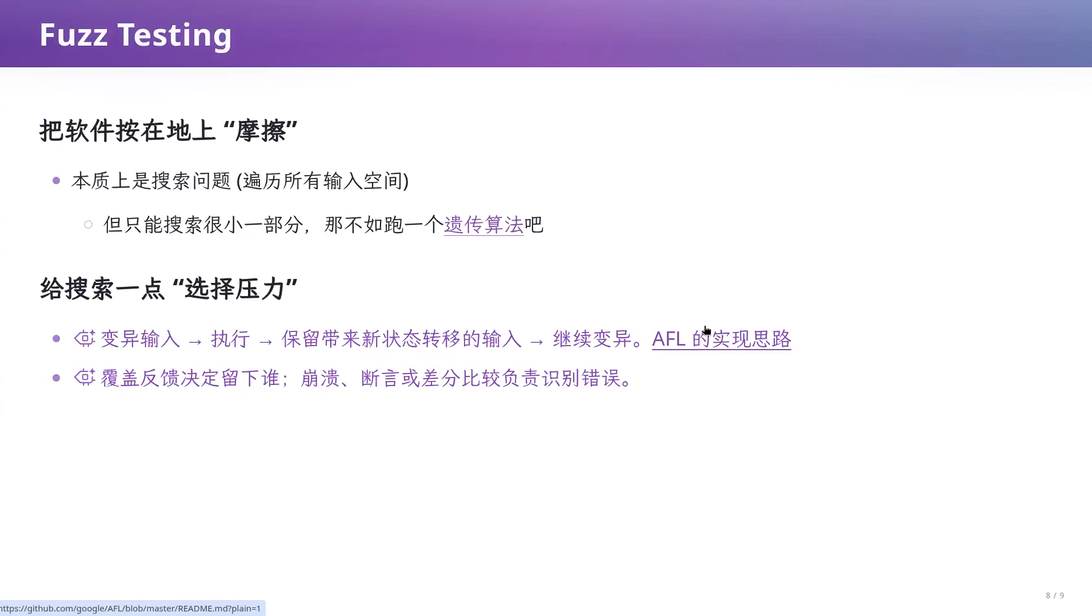
\includegraphics[width=0.92\textwidth]{figures/fig_41_fuzz_testing_afl_genetic.png}
\caption{模糊测试（Fuzz Testing）：将输入空间遍历建模为搜索问题，利用 AFL 的边覆盖反馈赋予变异过程“遗传算法选择压力”\vtag}
\end{figure}
\srcnote{01:32:15--01:32:30}

为什么传统的纯随机模糊测试（Black-box Random Fuzzing，即往程序里乱塞一通随机字节流）效率很低？因为真实程序（如解析 PNG 图片、ELF 二进制或 SQL 语句的解析器）往往在入口处有一层层严格的格式校验（例如检查文件头前 4 个字节是否等于魔数 \texttt{0x89 'P' 'N' 'G'}）。纯随机生成的字节流有 $1 - 2^{-32} \approx 99.99999998\%$ 的概率在第一行校验就被直接拒绝返回错误，根本进不到程序深层的核心状态空间！

**AFL（American Fuzzy Lop）的“灵光一闪”在于：既然无法穷尽输入空间，不如把测试输入生成变成一场带“自然选择压力”的达尔文遗传演化算法（Genetic Algorithm）！**

\begin{equation}
\mathcal{Q}_{t+1}
= \mathcal{Q}_t \;\cup\;
\Big\{\, x' \in \mathrm{Mutate}(x) \;\Big|\; x \in \mathcal{Q}_t,\;\; \mathrm{CovEdges}(x') \not\subseteq \bigcup_{z \in \mathcal{Q}_t} \mathrm{CovEdges}(z) \,\Big\}
\end{equation}

上式刻画了 AFL 简洁到极致的核心循环：
\begin{enumerate}
    \item \textbf{轻量级插桩记录边覆盖（Edge Coverage）}：在编译被测程序时，编译器在每个基本块（Basic Block）跳转处插入几条汇编指令，记录本次运行走过了哪些控制流转移边 $\mathrm{CovEdges}(x)$；
    \item \textbf{随机变异（Mutation）}：从当前种子队列 $\mathcal{Q}_t$ 中取出一个输入 $x$，对其进行比特翻转（Bit Flip）、字节增删、边界整数替换、拼接等随机变异，生成一批子代输入 $x'$；
    \item \textbf{覆盖反馈提供“选择压力（Selection Pressure）”}：大多数变异出来的子代 $x'$ 走的还是老路，执行完直接丢弃；但**一旦某个变异体 $x'$ 歪打正着触发了一条以前所有种子都从未走过的新分支或新状态转移（即 $\mathrm{CovEdges}(x')$ 带来了新覆盖）**，AFL 就会眼前一亮：“这个输入有前途！”并立即将其保留进种子库 $\mathcal{Q}_{t+1}$，作为下一轮继续变异的跳板！
\end{enumerate}

通过这种“保留带来新状态转移的种子 $\to$ 在此基础上继续变异”的正反馈循环，AFL 甚至能在最初只给一个写着 \texttt{"hello"} 的文本文件的情况下，经过几小时的演化自己“猜”出合法的 JPEG 文件头或 XML 语法结构，一路钻进代码最深处的角落！而且请注意：**覆盖反馈（决定留下哪个输入继续变异）与错误判定（通过崩溃 Crash、AddressSanitizer 内存越界检查、内部 \texttt{assert} 断言或 DiffTest 差分比较来识别 Bug）是完全正交的**，两者一结合，就构成了现代系统软件最强大的自动找 Bug 机器。

\begin{knowledgebox}{Fuzzing 架构公式：覆盖反馈（探索方向）$\times$ 测试神谕（错误判定）}
现代高强度自动化测试的本质，就是将两个正交组件拼装成高速运转的搜索闭环：
\begin{itemize}
    \item \textbf{输入生成器（Fuzzer / 遗传变异 $+$ 边覆盖反馈）}：负责在指数级输入空间中自动爬山，专挑能触发新控制流边（Edge Coverage）的输入留下继续变异，强力推动 $\mathtt{Fault \to Error}$；
    \item \textbf{错误检测器（Sanitizers / Assertions / DiffTest）}：在被测程序内部开启 \texttt{ASan/UBSan/TSan}、注入业务不变量 \texttt{assert} 或挂载参考模型 DiffTest，确保一旦变异输入触发了内部错误状态，立即转化为可捕获的 $\mathtt{Failure}$。
\end{itemize}
\end{knowledgebox}

\subsection{跳出屏幕的闭环测试：San Mehat 的 SD 卡插拔机器人与全讲总结}

到了全课的压轴环节，蒋老师分享了一个他个人最喜爱的、跳出电脑屏幕之外的工程测试故事——来自 Android 初创团队核心系统工程师 **San Mehat** 的回忆（幻灯片第 25 页，图 42）：

\begin{figure}[H]
\centering
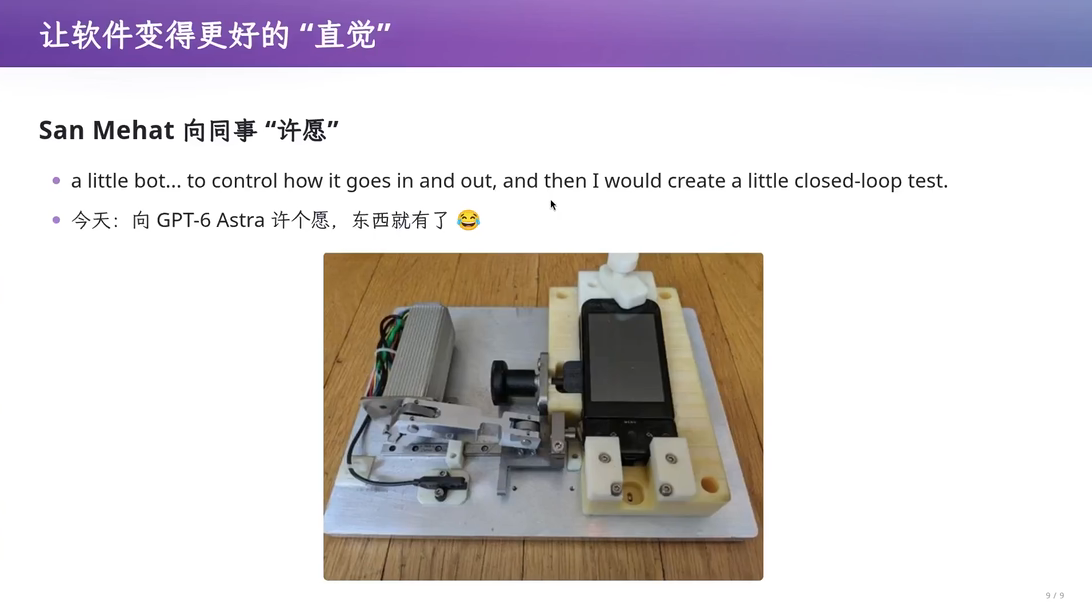
\includegraphics[width=0.92\textwidth]{figures/fig_42_san_mehat_sdcard_robot.png}
\caption{让软件变得更好的“直觉”：Android 初创团队工程师 San Mehat 向同事“许愿”打造一台由软件控制的 SD 卡自动插拔机械装置，构建软硬件物理闭环测试\vtag}
\end{figure}
\srcnote{01:36:00--01:36:15}

当年在研发世界上第一款 Android 手机（HTC Dream / T-Mobile G1）时，团队发现 Linux 内核自带的 SD 卡插槽驱动与 FAT 文件系统在用户频繁插拔 SD 卡时极不稳定（后来他们甚至被迫重写了整套驱动）。但这个问题在当时几乎无法用纯软件模拟器（如早期尚不成熟的 QEMU）复现，因为真实的物理拔卡伴随着金属触点的毫秒级机械抖动、供电跌落以及恰好发生在文件系统写入一半时的异步硬件中断；而如果雇一个测试员坐在工位上用手不停地拔插 SD 卡，不仅一天拔不了几百次，而且一旦触发内核崩溃，根本无法记录并重现刚才拔卡的精确毫秒时机！

面对这个死局，San Mehat 向身边懂硬件的同事“许了个愿”：
\begin{quote}
\textit{``Can you build me a little bot... to control how it goes in and out, and then I would create a little closed-loop test?''}\\
——**“你能不能帮我用 3D 打印和舵机做个小机器人，由我的测试程序发信号控制它把 SD 卡拔出来、插进去？这样我就能写一个全自动的闭环测试（Closed-Loop Test）了！”**
\end{quote}

看图 42 右侧那台由步进电机、连杆与电路板组成的精巧装置：当物理世界里不可控的“人手拔卡”被改造成了一个**受软件指令精确控制的舵机执行器**后，测试脚本就可以在昼夜不停的循环里执行：“发起大文件写入 $\to$ 等待 $17\,\mathrm{ms}$ $\to$ 发送脉冲命令舵机拔出 SD 卡 $\to$ 检查内核是否 Panic $\to$ 重新推入 SD 卡挂载验证文件系统一致性”！原本需要碰运气的物理故障，瞬间变成了可编程、可遍历、可复现的确定性闭环测试！

在课程的最后两分钟，蒋老师还微笑着拿出了自己钥匙扣上的一个小物件——那是他前一天刚刚结合家里小朋友的设计，向 AI 许愿生成的一个 **5厘米 $\times$ 5厘米 的四帧光栅画（Lenticular Animation）3D 打印卡扣相框**：只要给程序传入一张四帧动图，AI 写的脚本就能自动完成光栅条纹交织切片与卡扣外壳建模，拉动滑片时就会呈现出流畅的四帧动画效果，而且随时可以拉开卡扣更换里面 5厘米 $\times$ 5厘米 的相片。

\begin{importantbox}{全讲终极结语：今天所有东西都可以“许愿”，但许愿的前提是你有正确的概念！}
从 1996 年 Ariane 501 火箭的 16位整数溢出、1999 年火星气候轨道器的单位失配，到 2013年 NEMU 的 DiffTest、香山处理器的 4 亿周期验证、AFL 的覆盖引导演化，再到 San Mehat 的 SD 卡插拔机器人与今天的 \texttt{CS:THREE} 长程任务：
\begin{itemize}
    \item \textbf{AI 还干不了你认知边界之外的事情}：如果你脑子里没有“纯函数状态机与渲染分离”的架构概念，Agent 就会傻乎乎地靠截屏测 CS:GO 直到撞上 HTTP 413；如果你脑子里没有“差分测试（DiffTest）”或“覆盖引导模糊测试（Fuzzing）”的概念，你面对几十万行复杂系统就只能望洋兴叹。
    \item \textbf{成为为 AI 提供认知与闭环的领域专家}：在代码编写成本趋近于零的生成式软件工程时代，人类工程师最核心的价值，就是运用对 \texttt{Fault-Error-Failure}、可测试性架构、差分神谕与软硬件闭环的深刻洞察，向 AI 许下那个“真正切中工程命脉的愿望”。
\end{itemize}
\end{importantbox}

\subsection{本章小结}

本章剖析了模糊测试（Fuzz Testing）如何通过 AFL 边覆盖反馈将输入空间搜索转化为带选择压力的遗传算法，并通过 San Mehat 的 Android SD 卡自动插拔机器人与 5厘米 $\times$ 5厘米四帧光栅画钥匙扣案例，升华了“用正确工程概念指导 AI 许愿并构建自动化验证闭环”的课程主旨。

% =========================================================================
% END OF NOTES SUMMARY TABLE
% =========================================================================
\newpage
\section*{全讲核心知识点与自检清单}

\begin{table}[H]
\centering
\small
\caption{第 11 讲《软件质量保障 (1)》核心概念、数学模型与工程范式速查表}
\begin{tabular}{p{2.8cm}p{4.6cm}p{5.9cm}}
\toprule
\textbf{知识模块} & \textbf{核心概念 / 历史案例} & \textbf{生成式软件工程实战准则} \\
\midrule
\textbf{演化与自动化反讽} & \texttt{intent-spec-impl gap}、Git Rebase 学习法、Bainbridge（1983）自动化的反讽 & 警惕“能跑但失控”的许愿陷阱；日常不练手会导致异常接管兜底时彻底丧失心智模型 \\
\textbf{程序员幻觉与 UB} & 10年前 \texttt{nvbn/thefuck}、双层循环 \texttt{j++} 误写为 \texttt{i++}、有符号溢出 UB & 绝不相信人类或 AI 仅凭“感觉”写出的几百行代码；警惕 $n=0$ 掩盖缺陷与编译器激进优化 \\
\textbf{质量三元因果链} & \texttt{Fault}（缺陷）$\to$ \texttt{Error}（内部脏状态）$\to$ \texttt{Failure}（外部失效）、Ariane 501（16位越界） & 明确观察边界（如 0.0001秒超时）；切记同构主备冗余会被同一确定性软件 Bug 同时击穿 \\
\textbf{测试与断言双轮} & Java / Safe Rust 预防、Testing（遍历规约） vs Assertion（即时检查） & 用测试推动 \texttt{Fault $\to$ Error}，在代码内部密集布置 \texttt{assert} 推动 \texttt{Error $\to$ Failure} 缩短潜伏期 \\
\textbf{广义输入与反馈} & \texttt{package-lock.json}、\texttt{gettimeofday()}（$T+1\text{秒}/1\text{毫秒}$）、CHESS、$1/n!$、2024年 \texttt{SWE-agent} & 跑 100次/1000次/1万次通过不代表跨环境与并发安全；利用 ACI 执行测试闭环赋能 Agent 自纠错 \\
\textbf{经典测试工程矩阵} & 100万行四层测试、火星轨道器、黑盒/白盒（100\%覆盖反例）、酒吧漫画、测试金字塔 & 接口连通后必查单位语义；严防无断言的虚假高覆盖率；回归测试必先确认修复前 Fail、修复后 Pass \\
\textbf{可测试性系统架构} & \texttt{CS:THREE}（202次提交/跑12秒交火/413报错）、纯函数、Stripe 幂等键、FoundationDB（100台） & 拒绝截屏测核心逻辑；用纯函数 $\mathrm{step}(S,a)$ 隔离渲染，显式注入时钟与随机种子实现确定性重放 \\
\textbf{差分测试 DiffTest} & 2013年 NEMU 调试《仙剑》跑飞、香山（XiangShan）运行 4 亿周期捕获 \texttt{mstatus} & 缺乏人工 Oracle 时，让两份独立实现逐指令锁步比对状态，在第一处分歧 $k^*$ 当场停机 \\
\textbf{模糊测试与软硬闭环} & 30年搜索难题、AFL 边覆盖遗传算法、San Mehat SD 卡机器人、5厘米光栅画钥匙扣 & 用覆盖率反馈赋予随机变异选择压力；将不可控的外部物理操作改造为软件可编程的闭环执行器 \\
\bottomrule
\end{tabular}
\end{table}

\end{document}
